\setcounter{chapter}{3} % previous chapter number

\chapter{Symmetry and periodicity in photonics}
\label{h:periodic}

\begin{quote}
The mathematical sciences particularly exhibit order, symmetry, and limitation; and these are the greatest forms of the beautiful.

--- Aristotle
\end{quote}

\begin{quote}
Attaching significance to invariants is an effort to recognise what, because of its form or colour or meaning or otherwise, is important or significant in what is only trivial or ephemeral. A simple instance of failing in this is provided by the poll-man at Cambridge, who learnt perfectly how to factorise $a^2 - b^2$ but was floored because the examiner unkindly asked for the factors of $p^2 - q^2$.

--- H.W. Turnbull
\end{quote}

%$$\setcounter{page}{1}
\minitoc

Systems which exhibit symmetry and periodicity are important in photonics, as e.g. in so--called photonic crystals, which are artificial media where the refractive index has a periodicity on a scale of the order of the wavelength. This chapter introduces some concepts which are important for the study of these systems.

First, the scalar Helmholtz equation will be generalised to a vectorial equation which can also be used in the case of continuous index variations. We will interpret this as an eigenvalue problem, introduce the concept of a Hermitian operator and discuss some of its properties.

Next, we will analyse how we can use symmetries in these systems to classify modes. A very important symmetry is that of a discrete translational symmetry or periodicity. This will allow us to talk about Bloch's theorem, Brillouin zones and band diagrams. 

Finally, we will discuss some applications of photonic crystals, and show how they can be used to localise light in a cavity, or guide it along a waveguide.

\section{The vectorial Helmholtz equation in non--uniform media}

\subsection{The Helmholtz equation as an eigenvalue problem}

We will first derive the most general form of the Helmholtz equation which is also valid in the case of continuous refractive index variations. We start from

\begin{equation}
\nabla \times {\bf E({\bf r})} = - j \omega \mu {\bf H({\bf r})} \label{eq-maxwell-1}
\end{equation}
\begin{equation}   
\frac{1}{\varepsilon({\bf r})}\nabla \times {\bf H({\bf r})} = j \omega {\bf E({\bf r})} \label{eq-maxwell-2}
\end{equation}

Direct substitution of Eq.~\ref{eq-maxwell-2} into Eq.~\ref{eq-maxwell-1} yields

\begin{equation}
\fbox{$\displaystyle
\nabla \times \left[ \frac{1}{\varepsilon({\bf r})}\nabla \times {\bf H({\bf r})}  \right ] = \omega^2 \mu {\bf H({\bf r})} \label{eq-master}
$}
\end{equation} 

It is important not to yield to the temptation of bringing $\varepsilon({\bf r})$  outside of the $\nabla$--operator. This would be incorrect, because $\varepsilon$ is now no longer constant (although we assume that $\mu$ is constant since most 'normal' materials are non--magnetic).

Let's define the following linear differential operator:

\begin{equation}
\Theta \stackrel{def}{=} \nabla \times  \frac{1}{\varepsilon({\bf r})}\nabla \times
\end{equation} 

This operator takes the curl, divides by $\varepsilon({\bf r})$ and then takes the curl again. Using this notation, we can easily write Eq.~\ref{eq-master} as an eigenvalue problem:

\begin{equation}
\Theta {\bf H({\bf r})} = \omega^2 \mu {\bf H({\bf r})}
\end{equation} 

So, the eigenfunctions ${\bf H({\bf r})}$ of the $\Theta$--operator are field distributions that satisfy Maxwell's curl equations. The eigenvalues of these eigenfunctions are given by $\omega^2 \mu$. Note that in this point of view $\omega$ is seen as an unknown: for a given system with a certain index distribution, we are interested in finding the  $\omega$--values of the allowed solutions.

For physical reasons, we would obviously like these eigenvalues to be real and positive, as that would give rise to a real and positive value of the angular frequency $\omega$, provided that $\mu$ is real and positive.

To prove this, one of the concepts that we will need to use is that of \emph{Hermitian} operators.

\subsection{Hermiticity}

To define what it means for an operator to be Hermitian, we first need to introduce a scalar product (also called inner product). Let's define this inner product between two vector functions ${\bf F({\bf r})}$ and ${\bf G({\bf r})}$ as

\begin{equation}
\fbox{$\displaystyle
\left\langle {\bf F}, {\bf G}\right\rangle = \iiint {\bf F^*({\bf r})} \cdot {\bf G({\bf r})} dV
$}
\end{equation} 

From this simple definition. we immediately get that $\left\langle {\bf F}, {\bf G}\right\rangle = \left\langle {\bf G}, {\bf F}\right\rangle ^*$. We also see that $\left\langle {\bf F}, {\bf F}\right\rangle$ is always real, even if ${\bf F}$ itself is complex.

Now, an operator $\Xi$ is said to be Hermitian if

\begin{equation}
\fbox{$\displaystyle
\left\langle {\bf F}, \Xi {\bf G}\right\rangle = \left\langle \Xi {\bf F}, {\bf G}\right\rangle
$}
\end{equation} 

This means that it doesn't matter which function is operated upon before taking the inner product. Clearly this is a special property which not all operators have. Before showing that our operator $\Theta$ has this property, let's first derive an auxiliary result to help us manipulate the integrals involved in taking the scalar product. 

Starting from

\begin{equation}
\nabla \cdot ({\bf a} \times {\bf b}) = {\bf b} \cdot ( \nabla \times {\bf a}) - {\bf a}  \cdot (\nabla \times {\bf b})
\end{equation} 

we immediately get

\begin{equation}
\iiint {\bf a}  \cdot (\nabla \times {\bf b}) dV = \iiint {\bf b} \cdot ( \nabla \times {\bf a}) dV - \iiint \nabla \cdot ({\bf a} \times {\bf b}) dV 
\end{equation} 

With the divergence theorem, this can be written as

\begin{equation}
\iiint {\bf a}  \cdot (\nabla \times {\bf b}) dV = \iiint {\bf b} \cdot ( \nabla \times {\bf a}) dV - \iint  {\bf a} \times {\bf b} \cdot d{\bf S} \label{eq-part-int}
\end{equation} 

Now, back to our proof of the hermiticity of $\Theta$. Simply applying definitions, we get

\begin{equation}
\left\langle {\bf F}, \Theta {\bf G}\right\rangle = \iiint {\bf F}^* \cdot\nabla \times \left[ \frac{1}{\varepsilon({\bf r})}\nabla \times {\bf G({\bf r})}  \right ] dV 
\end{equation} 

By applying our lemma Eq.~\ref{eq-part-int}, we get

\begin{equation}
\left\langle {\bf F}, \Theta {\bf G}\right\rangle = \iiint [ \nabla \times {\bf F}]^* \cdot \left[ \frac{1}{\varepsilon({\bf r})}\nabla \times {\bf G({\bf r})}  \right ] dV 
\label{eq-pos-omega}
\end{equation} 

The term related to the surface integral was dropped because in all practical cases, one of two things will be true. Either the fields at infinity will decay to zero, or the fields are periodic on the surface. In both cases, the surface term will vanish.

If $\varepsilon$ is real (which will be the case for lossless media), we can write

\begin{equation}
\left\langle {\bf F}, \Theta {\bf G}\right\rangle = \iiint \left [\frac{1}{\varepsilon({\bf r})} \nabla \times {\bf F}\right]^* \cdot \left[ \nabla \times {\bf G({\bf r})}  \right ] dV 
\end{equation} 

Applying our lemma Eq.~\ref{eq-part-int} one more time, we get

\begin{equation}
\left\langle {\bf F}, \Theta {\bf G}\right\rangle = \iiint \left[ \nabla \times  \left [\frac{1}{\varepsilon({\bf r})} \nabla \times {\bf F}\right] \right ] ^* \cdot {\bf G({\bf r})}  dV  = \left\langle \Theta {\bf F}, {\bf G}\right\rangle 
\end{equation} 

This proves that our operator is indeed Hermitian.

\begin{sidebar}
\begin{ex}
In this exercise, we will explore the relation between Hermitian operators and Hermitian matrices. As an operator working on a function, we take a matrix ${\bf A}$ which multiplies a column vector ${\bf x}$, i.e. the effect of the operator is given by ${\bf A} \cdot {\bf x}$. Let us define the scalar product between two column vectors as

$$\left\langle {\bf x},{\bf y} \right\rangle \stackrel{def}{=} {\bf x}^H \cdot {\bf y} = \sum{x_i^* y_i}$$

Now show that the operator defined by matrix multiplication by ${\bf A}$ is Hermitian if the matrix ${\bf A}$ is Hermitian, i.e. ${\bf A} = {\bf A}^H$.
\end{ex}
\end{sidebar}

\begin{sidebar}
\begin{ex}
From Maxwell's curl equations, derive an eigenvalue problem for the electric field. Show that even in lossless media, the resulting operator is not Hermitian, which is why people often prefer a representation in terms of the magnetic field.
\end{ex}
\end{sidebar}


\subsection{Properties of a Hermitian operator}

\subsubsection{Real eigenvalues}

Let's return to our eigenvalue problem:

\begin{equation}
\Theta {\bf H} = \omega^2 \mu {\bf H}
\end{equation} 

Taking the inner product of this equation with ${\bf H({\bf r})}$, we get

\begin{equation}
\left\langle{\bf H} , \Theta {\bf H}\right\rangle  = \omega^2 \mu \left\langle {\bf H} , {\bf H}\right\rangle \label{eq-real-eigen-1}
\end{equation}

Now, taking the complex conjugate and using the fact that $\left\langle {\bf F}, {\bf F}\right\rangle$ is always real, we get

\begin{equation}
\left\langle{\bf H} , \Theta {\bf H}\right\rangle^*  = (\omega^2 \mu)^* \left\langle {\bf H} , {\bf H}\right\rangle 
\end{equation} 

For any operator $\left\langle {\bf G}, {\bf F}\right\rangle ^*  = \left\langle {\bf F}, {\bf G}\right\rangle$ such that

\begin{equation}
\left\langle \Theta {\bf H} , {\bf H} \right\rangle  = (\omega^2 \mu)^* \left\langle {\bf H} , {\bf H}\right\rangle 
\end{equation} 

But $\Theta$ is Hermitian, so we can write

\begin{equation}
\left\langle {\bf H} , \Theta {\bf H} \right\rangle  = (\omega^2 \mu)^* \left\langle {\bf H} , {\bf H}\right\rangle \label{eq-real-eigen-2}
\end{equation} 

Comparing Eq.~\ref{eq-real-eigen-1} and Eq.~\ref{eq-real-eigen-2}, we get that $(\omega^2 \mu)^* = \omega^2 \mu$, so \emph{the eigenvalues of a Hermitian operator are real}. If we now only consider lossless materials with real $\mu$, it immediately follows that $\omega^2$ is real.

\subsubsection{Positive $\omega^2$}

Using a different argument, we can show that not only is $\omega^2$ real, it is also always positive. Setting ${\bf F}={\bf G}={\bf H}$ in Eq.~\ref{eq-pos-omega}, we get

\begin{equation}
\left\langle {\bf H}, \Theta {\bf H}\right\rangle = \iiint \frac{1}{\varepsilon({\bf r})} \left | \nabla \times {\bf H({\bf r})} \right |^2  dV 
\label{eq-rot-H-bis}
\end{equation} 

With Eq.~\ref{eq-real-eigen-1} this becomes

\begin{equation}
\omega^2 \mu \left\langle {\bf H} , {\bf H}\right\rangle = \iiint \frac{1}{\varepsilon({\bf r})} \left | \nabla \times {\bf H({\bf r})} \right |^2  dV \label{eq-omega-pos}
\end{equation} 

For lossless dielectrics $\varepsilon$ is real and positive. Since now all terms in Eq.~\ref{eq-omega-pos} are positive, $\omega^2$ must be positive too. So, we can pick the positive square root, leading to a positive $\omega$ and a physical interpretation.

Note that the fact that the eigenvalues are positive here, is due to the special form of our operator. It is \emph{not} a general property of Hermitian operators.

\subsubsection{Orthogonality}

Consider two modes ${\bf H}_1$ and ${\bf H}_2$ with frequencies $\omega_1$ and $\omega_2$. Because these are eigenfunctions of $\Theta$ we can write

\begin{equation}
 \left\langle {\bf H}_1 , \Theta {\bf H}_2\right\rangle = \omega_2^2 \mu \left\langle {\bf H}_1 , {\bf H}_2\right\rangle 
\label{eq-ortho-1}
\end{equation}

and

\begin{equation}
 \left\langle \Theta {\bf H}_1 , {\bf H}_2\right\rangle = \omega_1^2 \mu \left\langle {\bf H}_1 , {\bf H}_2\right\rangle
\label{eq-ortho-2}
\end{equation}

Because $\Theta$ is hermitian, the left--hand sides of Eq.~\ref{eq-ortho-1} and Eq.~\ref{eq-ortho-2} are equal, so we get

\begin{equation}
(\omega_2^2 - \omega_1^2) \left\langle {\bf H}_1 , {\bf H}_2\right\rangle = 0
\end{equation} 

If $\omega_1 \ne \omega_2$, we have $\left\langle {\bf H}_1 , {\bf H}_2\right\rangle = 0$ and we say that ${\bf H}_1$ and ${\bf H}_2$ are orthogonal modes.

In the special case where two different modes have the same frequency $\omega_1 = \omega_2$, we call them \emph{degenerate} modes\footnote{Note: solutions which only differ by a propertionality constant are not considered to be degenerate, but rather, they are considered to be the ``same'' mode.}, which are not necessarily orthogonal. However, since $\Theta$ is a linear operator, any linear combination of these degenerate eigenmodes will also be an eigenmode with the same frequency. This means that we can always choose to work with linear combinations that are orthogonal. These combinations can be obtained by e.g. a Gram--Schmidt orthogonalisation procedure.

\subsection{A variational form of the eigenvalue problem}

In order to get some general feeling for the nature of the modes and derive some more of their properties, it is useful to look at a variational form:

\begin{equation}
J \stackrel{def}{=} \frac{\left\langle {\bf H} , \Theta {\bf H}\right\rangle}{\left\langle {\bf H} , {\bf H}\right\rangle} \label{eq-variational}
\end{equation}  

We will show that any function ${\bf H}$ for which $J$ is stationary (i.e. $\delta J=0$) will satisfy our eigenvalue problem.

We can calculate the first variation of $J$ directly from Eq.~\ref{eq-variational}. However, it turns out that the calculation is a bit easier if we first rewrite Eq.~\ref{eq-variational} as

\begin{equation}
\left\langle {\bf H},{\bf H} \right\rangle J = \left\langle {\bf H},\Theta {\bf H} \right\rangle \label{eq-variational-1}
\end{equation} 

Replacing ${\bf H}$ by ${\bf H} + \delta {\bf H}$ and $J$ by $J+ \delta J$, we get:
\begin{equation}
\left\langle {\bf H+\delta {\bf H}},{\bf H}+\delta {\bf H} \right\rangle J + \left\langle {\bf H}+\delta {\bf H},{\bf H+\delta {\bf H}} \right\rangle \delta  J= \left\langle {\bf H}+\delta {\bf H},\Theta {\bf H} + \Theta \delta {\bf H} \right\rangle \label{eq-variational-2}
\end{equation} 

Subtracting Eq.~\ref{eq-variational-1} from Eq.~\ref{eq-variational-2} and neglecting higher order variations gives

\begin{equation}
\left\langle \delta {\bf H},{\bf H} \right\rangle J + \left\langle {\bf H},\delta {\bf H} \right\rangle J + \left\langle {\bf H}, {\bf H} \right\rangle \delta J = \left\langle {\bf H},\Theta \delta {\bf H} \right\rangle + \left\langle \delta {\bf H},\Theta {\bf H} \right\rangle \label{eq-variational-3}
\end{equation} 

\begin{sidebar}
\begin{ex}
Show that we can transform Eq.~\ref{eq-variational-3} to

$$\delta J = \frac {\left\langle \delta {\bf H} , {\bf G} \right\rangle + \left\langle {\bf G} , \delta {\bf H} \right\rangle}{2}$$

with

$${\bf G} \stackrel{def}{=} \frac{2}{\left\langle {\bf H} , {\bf H}\right\rangle } \left[ \Theta {\bf H} - \frac{\left\langle {\bf H} , \Theta {\bf H}\right\rangle}{\left\langle {\bf H} , {\bf H}\right\rangle} {\bf H} \right]  $$
\end{ex}
\end{sidebar}

Now, if $\delta J$ needs to be zero for all possible ${\delta \bf H}$, this means that ${\bf G}$ should be equal to zero, or

\begin{equation}
\Theta {\bf H} = \frac{\left\langle {\bf H} , \Theta {\bf H}\right\rangle}{\left\langle {\bf H} , {\bf H}\right\rangle} {\bf H} \label{eq-variational-4}
\end{equation} 

Bearing in mind that the quotient on the right hand side is just a number, Eq.~\ref{eq-variational-4} can only be fulfilled if ${\bf H}$ is indeed an eigenvector of $\Theta$. Incidentally, we have also proven that its eigenvalue is $J$.

Having survived the gory mathematical details of verifying that Eq.~\ref{eq-variational} is indeed variational, it's time to do something useful with it and derive a physical heuristic for the modes in our system.

First of all, let's evaluate $J$ for the case where ${\bf H}$ is a solution to the eigenvalue problem:

\begin{equation}
J =  \frac{\left\langle {\bf H} , \Theta {\bf H}\right\rangle}{\left\langle {\bf H} , {\bf H}\right\rangle} = \frac{\left\langle {\bf H} , \omega^2 \mu {\bf H}\right\rangle}{\left\langle {\bf H} , {\bf H}\right\rangle} = \omega^2 \mu
\end{equation}

This shows that solutions ${\bf H}$ which have low values of $J$ will tend to have a low frequency $\omega$.

Second, using Eq.~\ref{eq-rot-H-bis}, we can write the functional Eq.~\ref {eq-variational} as

\begin{align}
J =& \frac{1}{\left\langle {\bf H} , {\bf H}\right\rangle}  \iiint \frac{1}{\varepsilon({\bf r})} \left | \nabla \times {\bf H({\bf r})} \right |^2  dV  \label{eq-variational-HH}
\end{align} 

\begin{sidebar}
\begin{ex}
When ${\bf H}$ is a solution to the eigenvalue problem, transform Eq.~\ref{eq-variational-HH} into the following form, which contains only the electric field:
$$J=\frac{\iiint \left | \nabla \times {\bf E({\bf r})} \right |^2  dV} {\iiint \epsilon \left | {\bf E({\bf r})} \right |^2  dV} $$
\end{ex}
\end{sidebar}

From this equation, we can see that $J$ is minimised if the electric field ${\bf E}$ is concentrated in regions where the refractive index is high. So, to minimise $J$, a mode will try to concentrate its field in regions of high dielectric, while remaining orthogonal to the modes below it in frequency. With this heuristic we can e.g. explain why it is that dielectric waveguides do indeed work: the field likes to be concentrated in regions where the refractive index is high. Also, because of the link between $J$ and $\omega$, concentrating a mode in regions of high refractive index (thus lowering $J$) will tend to lower its frequency.

The same equation also suggests that to minimise $J$, is is advantageous to keep spatial variations in the field as low as possible so as to keep  $\left| \nabla \times {\bf E({\bf r})} \right |$ small. Indeed, the fundamental mode has much slower spatial variations than the higher order modes.

We will use these heuristics in a later section to explain the peculiar behaviour of certain periodic structures.

\begin{sidebar}
\begin{ex}
a) Show that, if you have two Hermitian operators $A$ and $B$, the generalised eigenvalue problem $A {\bf H} = \lambda B {\bf H}$ is the Euler-Langrange equation of the following variational expression: \\

$$J = \frac{\left\langle {\bf H} , A {\bf H}\right\rangle}{\left\langle {\bf H} , B {\bf H}\right\rangle}$$

What is $\lambda$? \\

b) Derive a generalised eigenvalue problem for {\bf E}. Is it Hermitian, i.e. are the two operators $A$ and $B$ involved in the generalised eigenvalue problem Hermitian? Note that it should be a true generalised eigenvalue problem, i.e. with $B$ not equal to the identity operator.  \\

c) Show based on the previous two results that minimising the following variational expression is equivalent to solving Maxwell's equations: \\

$$J=\frac{\iiint \left| \nabla \times {\bf E ({\bf r})} \right| ^2  dV} {\iiint \epsilon \left| {\bf E ({\bf r})} \right| ^2  dV}$$

\end{ex}
\end{sidebar}

\section{Using symmetries to classify modes}

In this section the use of symmetries to classify the solutions of Eq.~\ref{eq-master} is discussed.  A symmetry is a change of coordinates which leaves the form of Eq.~\ref{eq-master} intact.  

\begin{figure}
\centering
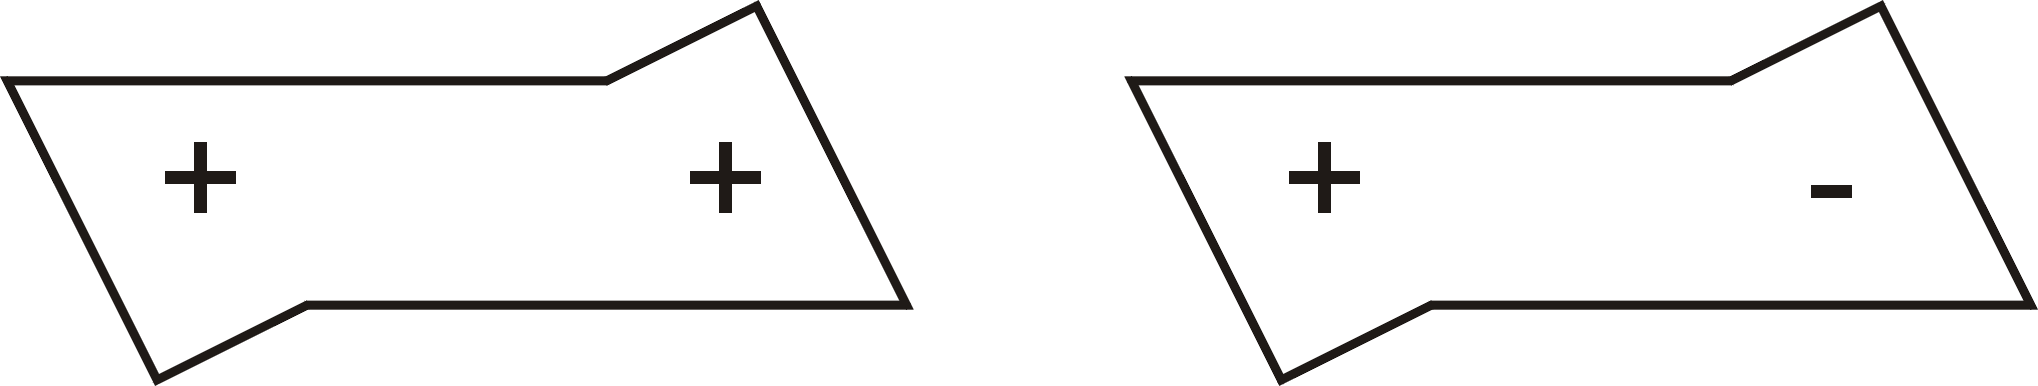
\includegraphics[width=8cm]{periodic/figures/symmcav}
\caption{A 2D metal cavity with inversion symmetry. On the left, an even mode with ${\bf H}({\bf r}) = {\bf H}(-{\bf r})$, on the right an odd mode with ${\bf H}({\bf r})=-{\bf H}(-{\bf r})$.}
\label{fig-symmcav}
\end{figure}

To clarify this, we start with the structure from Fig.~\ref{fig-symmcav}. This structure is inversion symmetric around its centre, i.e. invariant under the coordinate change ${\bf r}' = -{\bf r}$. Later in this section, we will consider other symmetries, like e.g. systems invariant under the transformation ${\bf r}' = {\bf r} + {\bf R}$, which is called translation symmetry.

\subsection{Inversion symmetry}

Suppose we want to find the modes of the cavity from Fig.~\ref{fig-symmcav}. Solving Maxwell's equations for such a cavity will not be possible analytically, but the cavity has an important symmetry: by inverting it about its centre, you end up with the same shape. So, if somehow we find that a particular pattern ${\bf H({\bf r})}$ is a mode of the cavity with frequency $\omega$, then ${\bf H({\bf -r})}$ must also be a mode with frequency $\omega$, since the cavity cannot tell ${\bf r}$ from ${\bf -r}$.

Now suppose ${\bf H({\bf r})}$ is not degenerate, so that it is the only mode at frequency $\omega$. Then, since ${\bf H({\bf -r})}$ is also a mode with frequency $\omega$, it must really be the same mode, which means that it must be a simple multiple of ${\bf H({\bf r})}$:

\begin{equation}
{\bf H({\bf -r})} = \alpha {\bf H({\bf r})}
\end{equation} 

To determine $\alpha$, we can invert the system twice, meaning that we return to the original function ${\bf H({\bf r})}$ and pick up another factor $\alpha$ in the process. So

\begin{equation}
\alpha^2 {\bf H({\bf r})} = {\bf H({\bf r})}
\end{equation} 

This means that $\alpha$ is either 1 or -1. So, a given nondegenerate mode \footnote{This is not true for degenerate modes. But, although we do not prove it here, we can always form new modes which \emph{are} even or odd, by taking appropriate linear combinations of degenerate modes.} must be one of two types: either it is invariant under inversion, ${\bf H({\bf -r})} = {\bf H({\bf r})}$, and we call it \emph{even}, or it becomes its own opposite, ${\bf H({\bf -r})} = - {\bf H({\bf r})}$ and we call it \emph{odd}.

So, we have classified the modes on how they respond to one of the cavity's symmetry operations. Let's place this on a slightly more mathematical footing. 

Suppose $O_I$ is an operator that inverts vector fields ${\bf H({\bf r})}$. Now, what is the mathematical expression that our system $\Theta$ has inversion symmetry? Since inversion is a symmetry of our system, it does not matter whether we operate with $\Theta$, or first invert the coordinates, then operate with $\Theta$ and then change the coordinates back:

\begin{equation}
\Theta = O_I^{-1} \Theta O_I
\end{equation} 

This can be rearranged as $O_I \Theta - \Theta O_I = 0$. Just like in quantum mechanics, we can define the \emph{commutator} $[A,B]$ of two operators $A$ and $B$ as

\begin{equation}
[A,B] \stackrel{def}{=} AB - BA
\end{equation} 

Note that the commutator is itself an operator. So, we have shown that our system is symmetric under inversion only if the inversion operator commutes with $\Theta$. If we now operate with this commutator on any mode ${\bf H({\bf r})}$ of the system, we get

\begin{equation}
[O_I, \Theta] {\bf H}= O_I(\Theta {\bf H}) - \Theta (O_I {\bf H} ) = 0
\end{equation} 

This means that

\begin{equation}
\Theta (O_I {\bf H} ) = O_I(\Theta {\bf H}) = O_I ( \omega^2 \mu {\bf H})
\end{equation} 

Or

\begin{equation}
\Theta (O_I {\bf H} ) =  \omega^2 \mu (O_I {\bf H})
\end{equation} 

This is nothing other than saying that if ${\bf H}$ is mode with frequency $\omega$, then $O_I {\bf H}$ is also a mode with the same frequency. But in the absence of degeneracy there can only be one mode per frequency, so ${\bf H}$ and $O_I {\bf H}$ can only differ by a multiplicative factor: $O_I {\bf H} = \alpha {\bf H}$. This is an eigenvalue equation for $O_I$, and we already know that the eigenvalues $\alpha$ are 1 and -1. 

Tracing back, we see that we started from a function ${\bf H}$ that was an eigenvector of $\Theta$ and ended up by showing that the same ${\bf H}$ was also an eigenvector of $O_I$ in the absence of degeneracy. 

But what if there is degeneracy in the system? In that case, two modes might have the same frequency, even though they are not related by a simple multiplier. Although we won't show it here, in that case it will still by possible to construct different linear combinations of these degenerate modes to make new modes which themselves are even or odd.

So, generally speaking, \emph{if two operators commute, it is possible to construct simultaneous eigenfunctions ${\bf H}$ of both operators}, i.e. functions ${\bf H}$ that are solutions of both eigenproblems $\Theta {\bf H} = \omega^2 \mu {\bf H}$ and $O_I {\bf H} = \alpha {\bf H}$.

This is very convenient, as eigenvectors and eigenvalues for simple symmetry operators can be easily determined, whereas those for $\Theta$ cannot. So we can classify the solutions according to the properties of the symmetry operation.

\begin{sidebar}
\begin{ex}
Given two linear operators $\bf A$ and $\bf B$, under which circumstances is

$$\left ( {\bf A} + {\bf B} \right ) ^2 =  {\bf A}^2 + 2 {\bf A}{\bf B}  + {\bf B}^2$$

For which exercise from chapter \ref{h:special} is this relevant?

\end{ex}
\end{sidebar}

\subsection{Continuous translation symmetry}

One way of saying that our system is unchanged by a translation over a displacement ${\bf d}$ is

\begin{equation}
\varepsilon ({\bf r} + {\bf d}) =  \varepsilon ({\bf r})
\end{equation} 

We can also define a translation operator $T_{\bf d}$:

\begin{equation}
T_{\bf d} \varepsilon ({\bf r}) \stackrel{def}{=} \varepsilon ({\bf r} + {\bf d})
\end{equation} 

Just like before, saying that our system in invariant under that operator amounts to $[\Theta, T_{\bf d}] = 0$.

A system with \emph{continuous} translation symmetry in the $z$--direction is invariant for all $T_{\bf d}$ in that direction. So, $\Theta$ must commute with all the translation operators over a distance ${\bf d} = d {\bf 1}_z$. In order not to make the notation too heavy, we will limit ourselves here to scalar fields which only vary in the $z$--direction.  We know that we can construct modes of $\Theta$ that are eigenfunctions of these translation operators $T_d$ as well:

\begin{equation}
T_d H(z) = H(z + d) = \lambda(d) H(z)
\end{equation} 

This has to be true for all possible $d$, but the eigenvalues $\lambda$ can be different for each $d$, which is why we write them as $\lambda(d)$. 

Geometrically it is obvious that a translation over $d$ followed by a translation over $d'$ is equivalent to a single translation over $d+d'$:

\begin{equation}
T_{d+d'}H(z) = T_{d'}T_{d}H(z)
\end{equation} 

This means that

\begin{equation}
\lambda(d + d')=\lambda(d')\lambda(d)
\end{equation} 

A function which has this property of converting sums to products is the exponential. Therefore there has to exist a number $k_z$ such that

\begin{equation}
\lambda(d) = e^{-j k_z d}
\end{equation} 

(The factor $-j$ is there to satisfy conventions.)

Therefore, we can write, for all possible $d$, 

\begin{equation}
H(z + d) = e^{-j k_z d}H(z) \label{eq-bloch-degenerate}
\end{equation} 

So, the $z$--dependence of the field can only be

\begin{equation}
H(z) = H_0 e^{-j k_z z}
\end{equation} 

Let's now take a closer look a two systems with continuous translation symmetry.

The first one is free space $\varepsilon({\bf r})=1$. This system has translation symmetry in all three dimensions. Following a similar line of reasoning as before, we conclude that the modes are of the form

\begin{equation}
{\bf H}_{\bf k}({\bf r}) = {\bf H}_0 e^{-j {\bf k} \cdot {\bf r}} \label{eq-plane-wave}
\end{equation} 

with ${\bf H}_0$ a constant vector. So, we have retrieved the plane wave solutions of Maxwell's equations based on symmetry arguments alone! Substituting the form of Eq.~\ref{eq-plane-wave} into Maxwell's equations, we can derive that $k^2 = \omega^2 / c^2$.


A second interesting system is that of a slab waveguide. In this case, the dielectric constant only varies on the $x$--direction and the system has continuous translation symmetry in the $z$-- and $y$--directions (Fig.~\ref{fig-slab-wg}). 

\begin{figure}[htb]
\centering
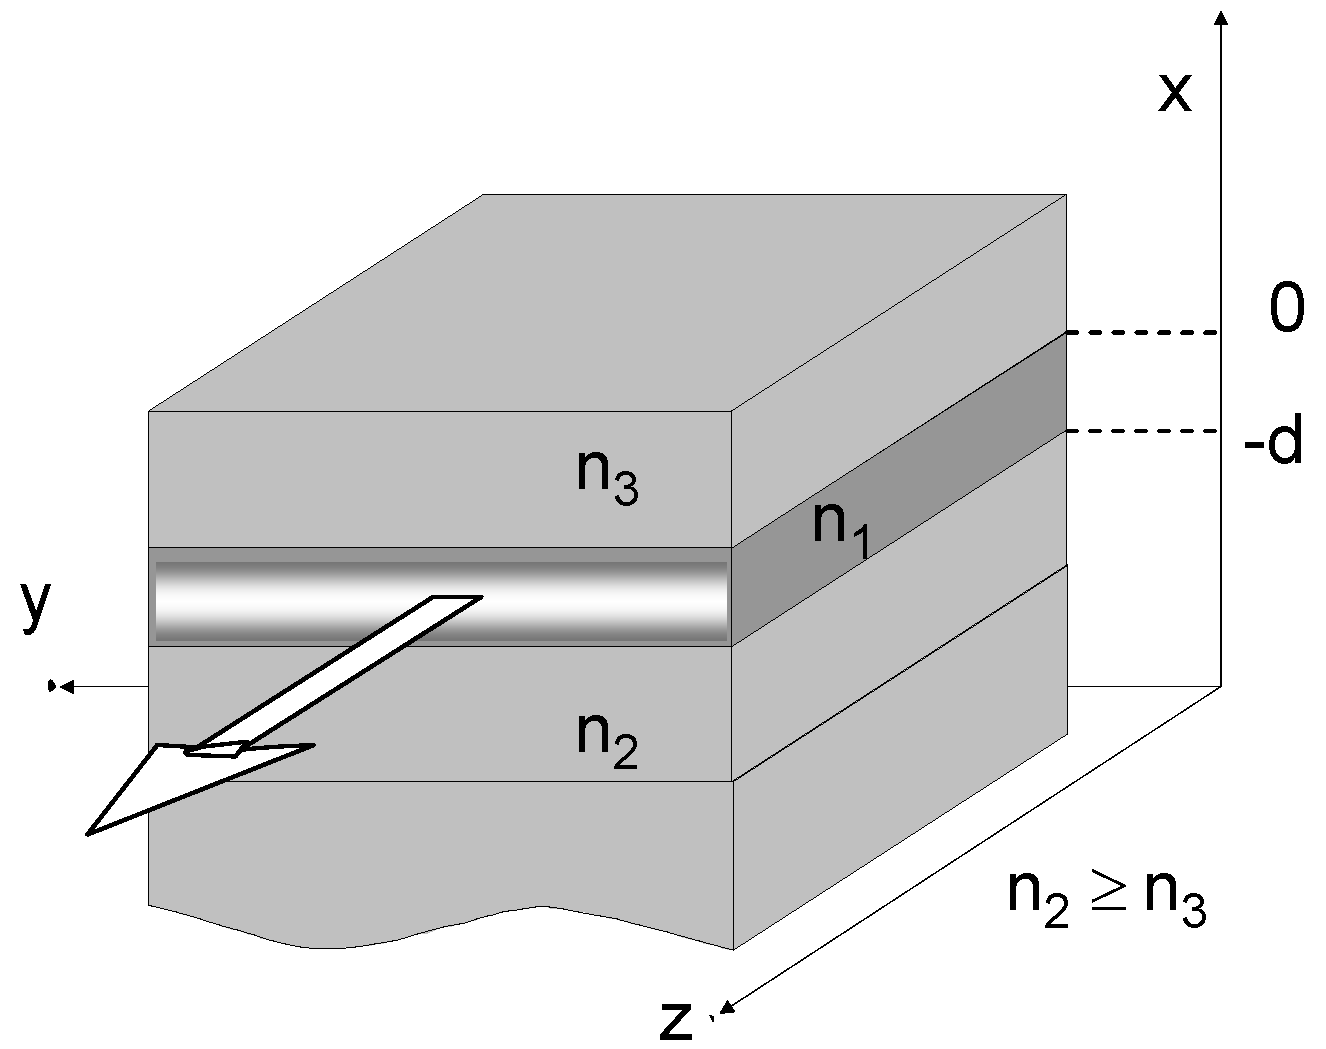
\includegraphics[width=7cm]{periodic/figures/slabwg}
\caption{Slab waveguide.}
\label{fig-slab-wg}
\end{figure}

This means the modes must have the following form:

\begin{equation}
{\bf H}_{\bf k}({\bf r}) = {\bf h}(x) e^{-j k_y y} e^{-j k_z z} 
\end{equation} 

Just like we did for the case of inversions, we can classify the modes by their eigenvalue of the symmetry operator, i.e. by their value of ${\bf k} = k_y {\bf 1}_y + k_z {\bf 1}_z$. Although we cannot say anything yet about ${\bf h}(x)$, we can nevertheless line up the modes in order of increasing frequency. For a given ${\bf k}$, we call $n$ the number indicating that mode's place in the line of increasing frequency, so we can identify each mode by its name $({\bf k},n)$.
$n$ is called the \emph{band number}\footnote{Don't confuse with the refractive index $n$.}. If there is a countable number of modes, $n$ is an integer, but sometimes $n$ may be a continuous variable. 

If we make a plot of wave vector versus frequency for the slab waveguide, the different bands correspond to different lines that rise uniformly in frequency. This \emph{band structure} is shown in Fig.~\ref{fig-slab-disp}\footnote{Beware that in some engineering texts this information is presented in a different way. Rather than plotting $\omega$ against $k$, $n_{eff}$ is plotted against $\lambda$, and such a plot is called a dispersion relation.}. It has been computed by solving Maxwell's equations numerically.

\begin{figure}
\centering
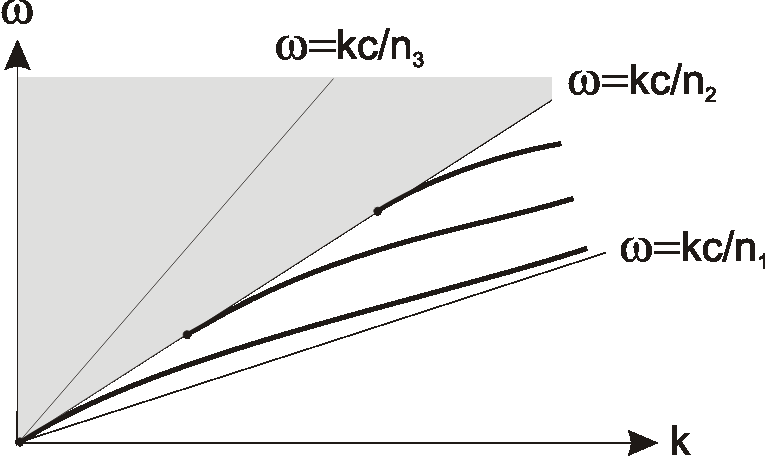
\includegraphics[width=7cm]{periodic/figures/slabdisp}
\caption{Dispersion relation of a slab waveguide.}
\label{fig-slab-disp}
\end{figure}

From e.g. the "Photonics" bachelor's course, we know that a slab waveguide has a discrete set of guided modes (which correspond to the lines in the band diagram), and also a continuous set of radiation modes (which corresponds to the shaded region in the band diagram). The boundary between these two sets of solutions is called the \emph{light line}.

The second variant of systems with translational symmetry, namely that of discrete translational symmetry is so important that it warrants its own section. We will start with 1D systems and later on move to higher dimensional systems.

\section{1D periodic systems}

\subsection{Discrete translational symmetry}

An important class of systems has \emph{discrete} translational symmetry, i.e. they are not invariant under translations of \emph{any} distance, but only under distances that are a multiple of some fixed step length.

Let's first study systems with such symmetry in one dimension. Higher dimensional systems will be discussed in the next section.

Fig.~\ref{fig-1d-periodic} shows a simple structure that is periodic in the $z$--direction, or - to phrase things differently - that has discrete translational symmetry in the $z$--direction. The basic step length is called the \emph{period} or the \emph{lattice constant} $a$, and the basic step vector is called the \emph{primitive lattice vector} ${\bf a} = a {\bf 1}_z$.

\begin{figure}[htb]
\centering
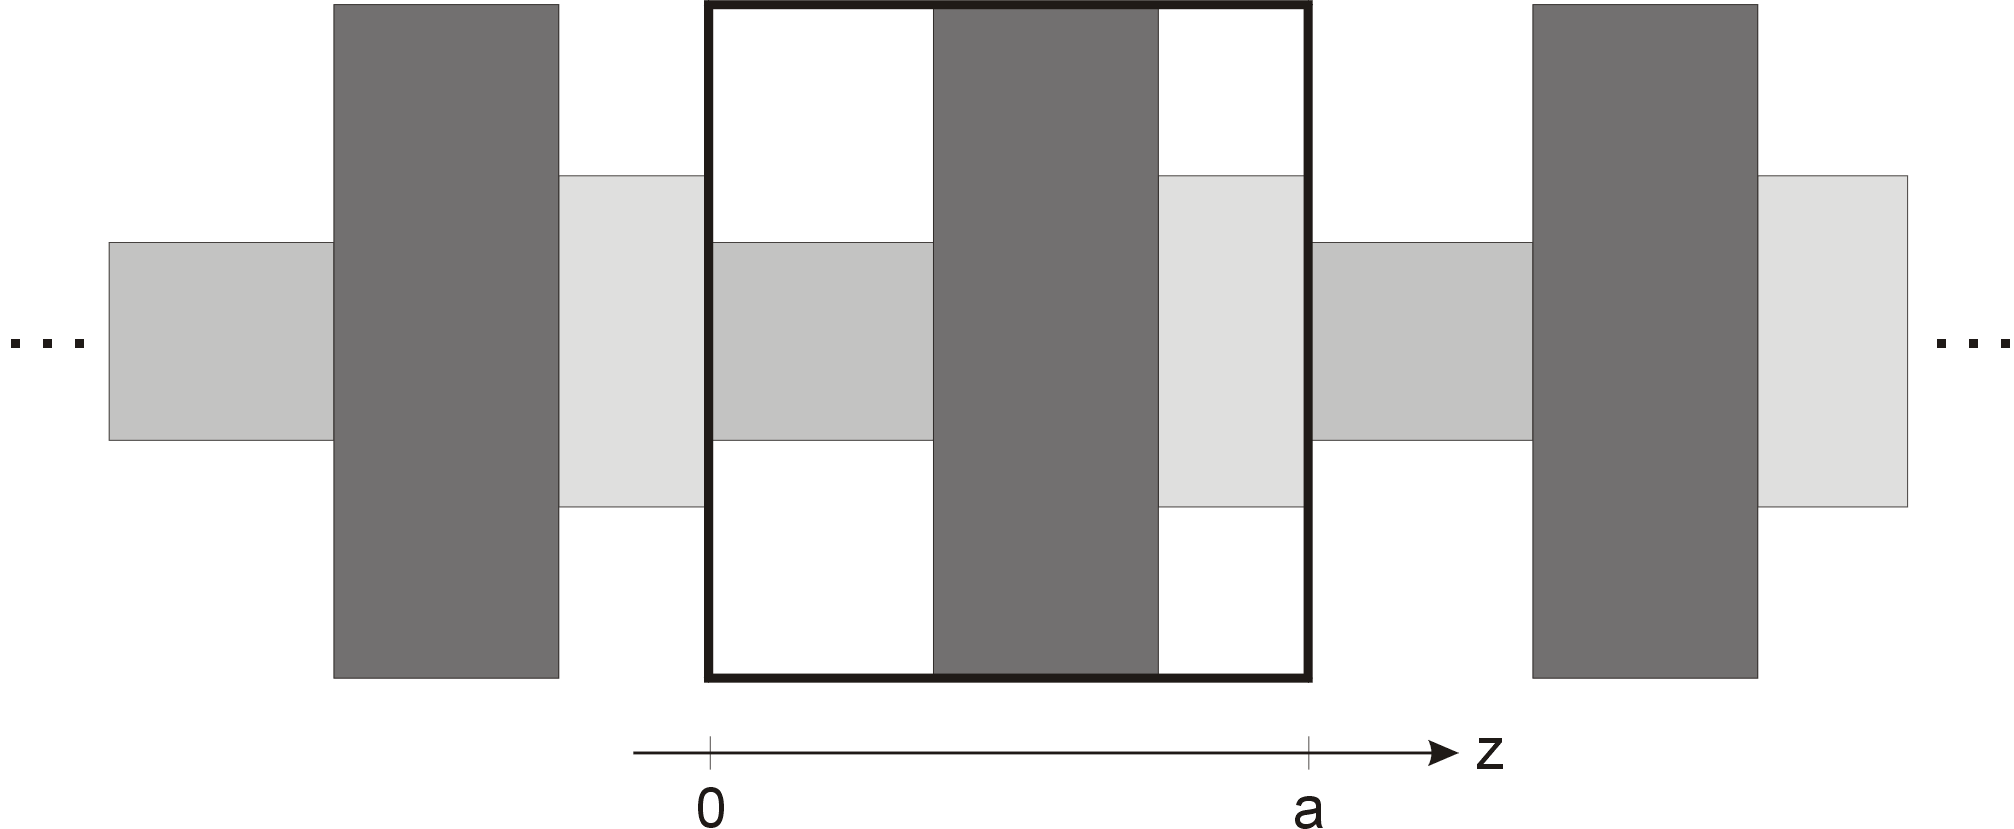
\includegraphics[width=9cm]{periodic/figures/periodic}
\caption{A 1D periodic structure with periodicity $a$ in the $z$--direction.}
\label{fig-1d-periodic}
\end{figure}

Because of symmetry, $\varepsilon({\bf r}) =  \varepsilon({\bf r} + {\bf a})$, or by repeating this procedure $\varepsilon({\bf r}) =  \varepsilon({\bf r} + l {\bf a})$ with $l$ an integer. The dielectric block that is considered to be repeated over and over is called the \emph{unit cell} and is highlighted in the square box in Fig.~\ref{fig-1d-periodic}. 

\subsection {Bloch's theorem}

We will now derive an important property of the eigenfunctions of systems with discrete translational symmetry.

Because of the symmetries present, $\Theta$ must commute with all the translation operators over a distance ${\bf R} = l a {\bf 1}_z$ in the $z$--direction. Again, we will restrict ourselves to the case of scalar fields only varying in the $z$--direction to lighten the notation.

We can follow the same argument that led to Eq.~\ref{eq-bloch-degenerate}, but this time with the set of translations over $la$, to arrive at

\begin{equation}
H(z + la) = e^{-j k_z la} H(z)
\end{equation} 

This leads to a first form of Bloch's theorem:

\begin{equation}
H(z + a) = e^{-j k_z a} H(z) \label{eq-bloch-1}
\end{equation} 

Note that this means that the Bloch mode itself is not periodic! Also, as mentioned before, a crucial difference with the case of continuous translation symmetry is that Eq.~\ref{eq-bloch-1} is only valid for displacements that are an integer multiple of the period, and not for arbitrary displacements.

Eigenfunctions of periodic systems are often called \emph{Bloch states}, and the number $k_z$ is called the \emph{wave number} of the Bloch state \footnote{Sometimes the name of Floquet is also used instead of that of Bloch. The mathematician Floquet first came up with this theory in the context of 1D systems in mechanics, while Bloch later generalised it to 3D in the context of solid state physics.}.

Once again, we can use this number $k_z$ to classify the modes and draw a band diagram. Compared to the case of continuous translational symmetry however, the wave number has a different interpretation. Rather than saying something about the phase relationship between any two different points on e.g. a slab waveguide, the Bloch wave number only provides a phase relationship between points in the structure that are spaced with the same periodicity as the system.

\subsection{Brillouin zone}

Looking at Eq.~\ref{eq-bloch-1}, it is clear that the wave number $k_z$ is only defined up to an integer multiple of $2 \pi/a$:

\begin{equation}
e^{-j (k_z + m\frac{2 \pi}{a} ) a} = e^{-j k_z a} e^{-j m 2 \pi} = e^{-j k_z a}
\end{equation} 

Any Bloch state doesn't have just a single wave number $k_z$ at a given frequency, but in fact a whole family of equivalent wave numbers $k_z+m 2 \pi /a$ at that frequency. This means that we can restrict our band diagram to e.g. the $k_z$--range $[-\pi/a,\pi/a]$. This important region of non--redundant $k_z$--values is called the \emph{Brillouin zone}. The band diagram at other $k_z$--values can be constructed by periodic repetition of the Brillouin zone (see Fig~\ref{fig-band-folding}).

\begin{figure}
\centering
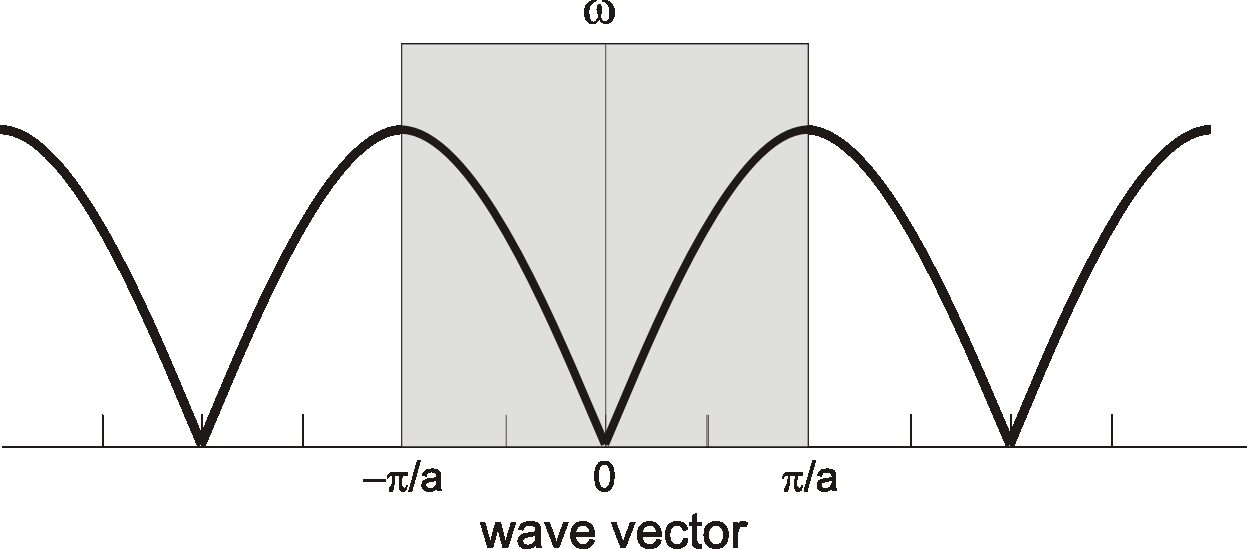
\includegraphics[width=10cm]{periodic/figures/band_folding}
\caption{Band structure of a periodic system. The Brillouin zone is the hatched region.}
\label{fig-band-folding}
\end{figure}

\subsection{A second form of Bloch's theorem}

Let's introduce a new function $u$:

\begin{equation}
u(z) = e^{j k_z z} H(z) \label{eq-bloch-u}
\end{equation} 

It is easy to prove that $u$ has the same periodicity of the lattice. We start from

\begin{equation}
u(z+la)= e^{j k_z z} e^{j k_z l a} H(z + l a)
\end{equation} 

With Eq.~\ref{eq-bloch-1} this becomes

\begin{equation}
u(z+l a)= e^{j k_z z} e^{j k_z l a} e^{-j k_z l a} H(z) = e^{j k_z z} H(z) = u(z)
\end{equation} 

Rewriting Eq.~\ref{eq-bloch-u}, we can say that the eigenfunctions of a 1D periodic system can be written as

\begin{equation}
H(z) = e^{-j k_z z} u(z) \label{eq-bloch-state}
\end{equation} 

with $u(z+l a) = u(z)$.

So, the solution $H(z)$ is a plane wave, as it would be in free space, but modulated by a periodic function because of the periodic lattice. This plane wave modulated by a periodic function is called a pseudoperiodic function.

Actually, since $u$ is periodic in $z$, we can write it as the following Fourier series:

\begin{equation}
u(z) =  \sum_{m=-\infty}^{\infty} u_m {e^{-j m \frac{2 \pi}{a} z}}
\end{equation} 

This means that

\begin{equation}
H(z)=  \sum_{m=-\infty}^{\infty} u_m {e^{-j \left( k_z + m \frac{2 \pi}{a} \right) z}}
\end{equation} 

This shows again that a Bloch mode is made up of an infinity of contributions with wave vectors $k_z + m 2 \pi / a$.

\begin{sidebar}
\begin{ex}
Consider a Bloch state $H(z)$ at frequency $\omega$ with wave vector $k$ and described by a certain periodic function $u_k(z)$ as per Eq.~\ref{eq-bloch-state}. The same Bloch state can also be described by another wave vector $k' = k+m 2 \pi / a$. What is the corresponding function $u_{k'}(z)$ for that description?
\end{ex}
\end{sidebar}

\subsection{Band gaps in 1D layered stacks}

As a simple example, let's plot the band diagram of a planar multilayered film, consisting of alternating layers of low index and high index materials, each with thickness $a/2$. This system is periodic in the $z$--direction, and Bloch theory tells us that we only need to consider $k_z$--values in the interval $-\pi / a \le k_z \le \pi / a$. As for $k_x$ and $k_y$, our system has continuous translation symmetry in these directions, so these $k$--components can assume any value. However, let's restrict ourselves now to the special case of normal incidence or on--axis propagation, where $k_x=k_y=0$. Without risk of confusion, we can abbreviate $k_z$ by $k$.

Let's first look at the case of zero index contrast between the materials, so that the medium is completely homogeneous. We already know that in such a system the solutions are plane waves with $\omega = c k / n$, so that one band is a straight line starting from the origin upwards toward the right. There is also a similar solution corresponding to waves propagating in the $-z$ direction instead of the $+z$ direction. This solution for negative values of $k=k_z$ is another straight line $\omega = - c k / n$ starting from the origin and going upwards toward the left. Now, we have imposed an artificial periodicity $a$ on this medium, which means that according to Bloch theory, these two lines should repeat themselves starting from the points $k = l 2 \pi / a$. This is illustrated in Fig.~\ref{fig-1d-bands-uniform}.

\begin{figure}
\centering
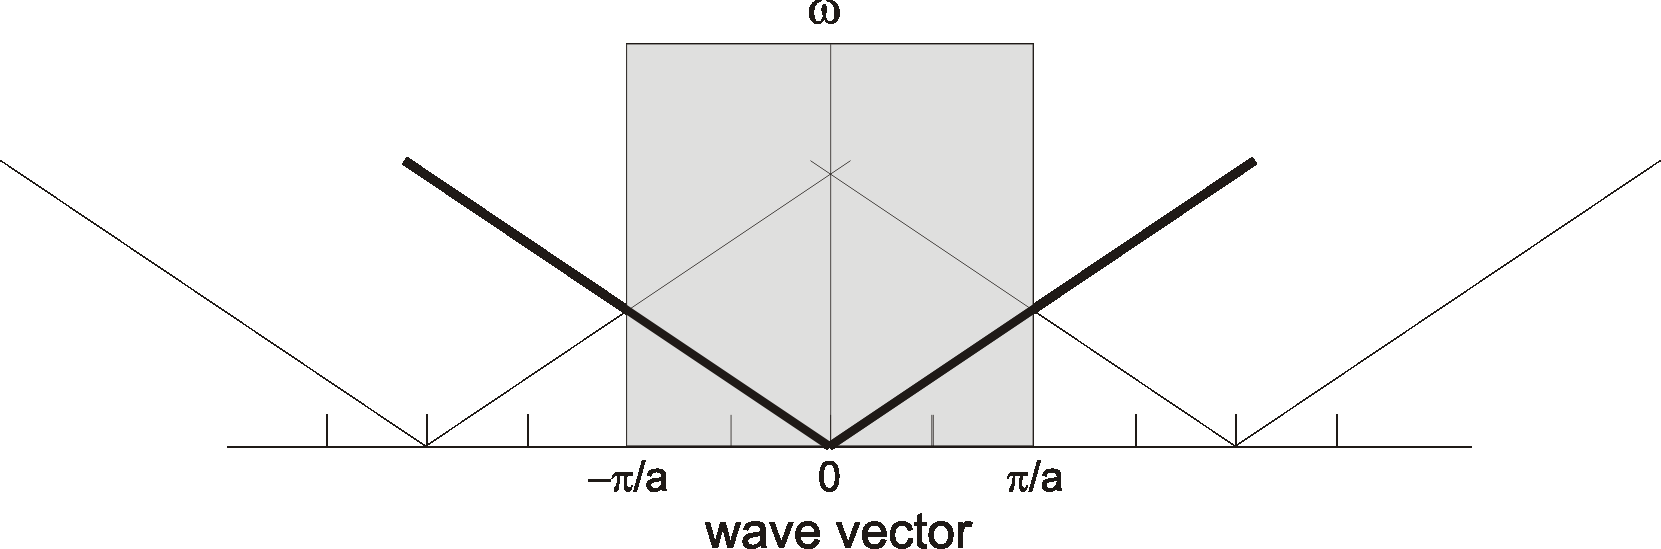
\includegraphics{periodic/figures/band_folding_uniform}
\caption{Band structures for a uniform medium where we impose an artificial periodicity $a$. The thick lines are the regular dispersion relations, the thin lines are copies of this as required by the artificial periodicity.}
\label{fig-1d-bands-uniform}
\end{figure}

When we restrict such a plot to the Brillouin zone, we get the results from the left panel of Fig.~\ref{fig-1d-bands}, with the bands appearing to fold back at the edges of the Brillouin zone. In this figure, we plot the band diagrams $\omega_n(k)$ for three different cases of index contrast between the two layers: zero, low and high.

\begin{figure}
\centering
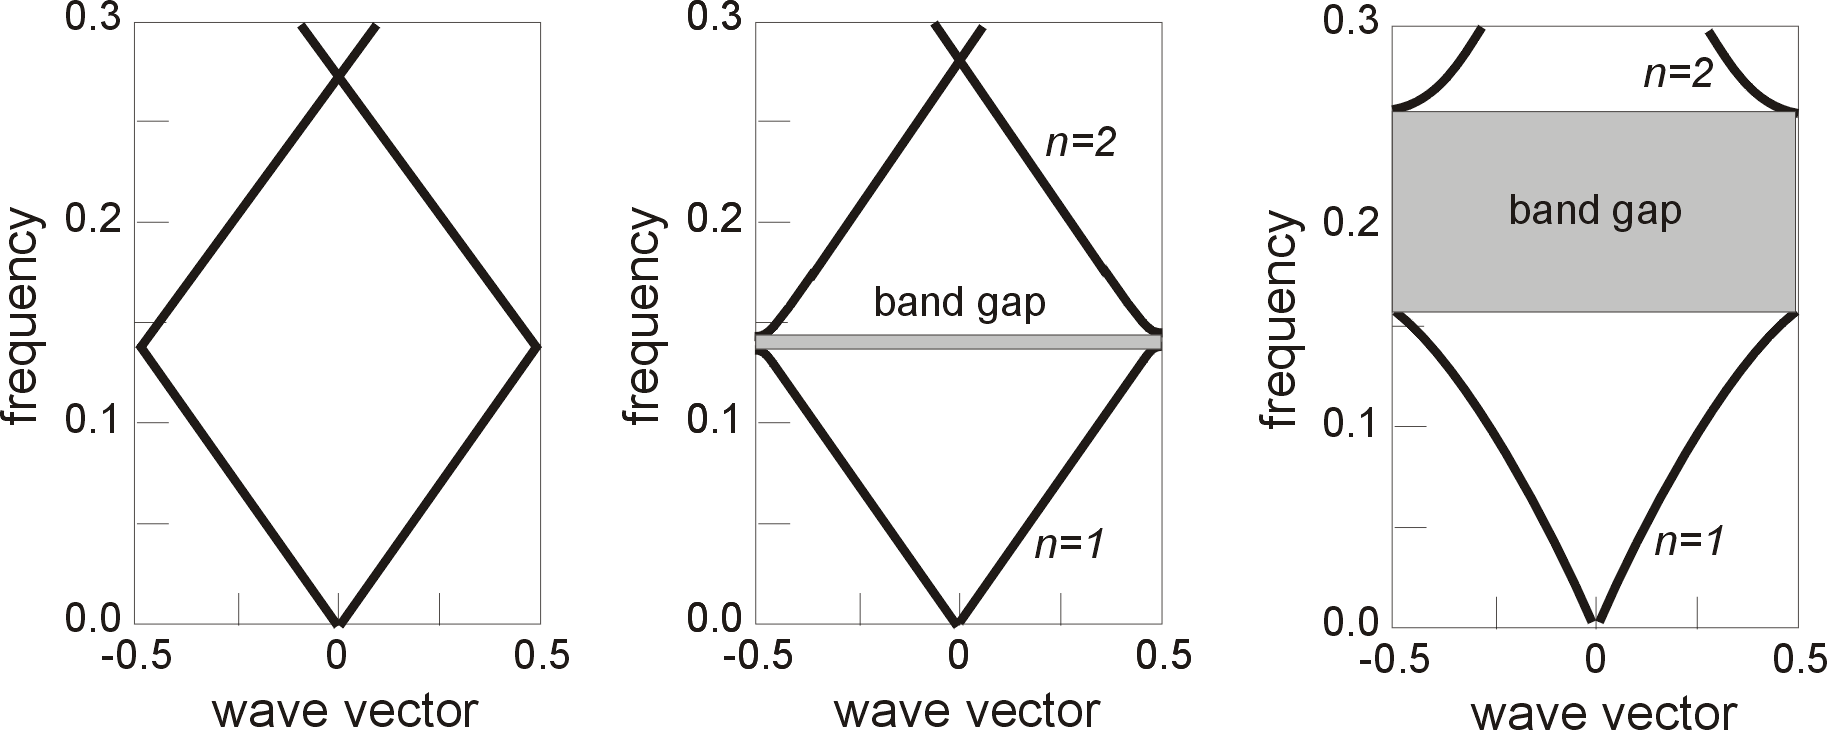
\includegraphics[width=12cm]{periodic/figures/1D_bands}
\caption{Band structures for normal incidence for three different multilayer films where all layers are $a/2$ thick. Left: all layers have $\varepsilon=13$. Middle: layers alternate between $\varepsilon=12$ and $\varepsilon=13$. Right: layers alternate between $\varepsilon=1$ and $\varepsilon=13$}
\label{fig-1d-bands}
\end{figure}

As we increase the index contrast, a curious feature emerges at the edges of the Brillouin zone in Fig.~\ref{fig-1d-bands}. We start to see frequency regions appear where no solutions exist for any $k$. This so--called \emph{photonic band gap} becomes wider as the index contrast increases.

What is the significance of such a band gap? In this frequency range, there are no allowed propagating states in the system. Suppose we have a semi--infinite periodic system for $z>0$, and a uniform medium for $z<0$. So, if we excite the semi--infinite periodic system with light coming from the uniform medium, this light will find no states to couple to inside the periodic system. Therefore, it has no choice but to return from where it came and be fully reflected. So, inside a band gap, a periodic structure acts as a perfect mirror.

Where does such a band gap come from? One way of explaining it, is saying that the reflections from each of the interfaces in the systems interfere constructively, such that the system will behave as a perfect reflector and no modes can exist inside it.

Another way of looking at it, is by making use of the heuristics we derived from the variational formulation of Maxwell's equations. Let's look at mode profiles for states immediately above and below the gap. The gap between bands 1 and 2 occurs at the edge of the Brillouin zone, where $k = \pi / a$. For this $k$--value, one can prove that the modes are standing waves with a wavelength of $\lambda = 2 \pi / k = 2a$, twice the lattice constant.

For small index contrast, one can also prove that the field profiles of the modes look like the ones in Fig.~\ref{fig-field-placement}. There are two ways to centre a standing wave of this kind, without violating the symmetry of the system: we can position its peak either in the low or in the high dielectric. But we know from our variational study that a mode that is more concentrated in high dielectric regions will have a lower frequency. So the two modes from Fig.~\ref{fig-field-placement} will have a different frequency and therefore a gap opens between them.

\begin{figure}
\centering
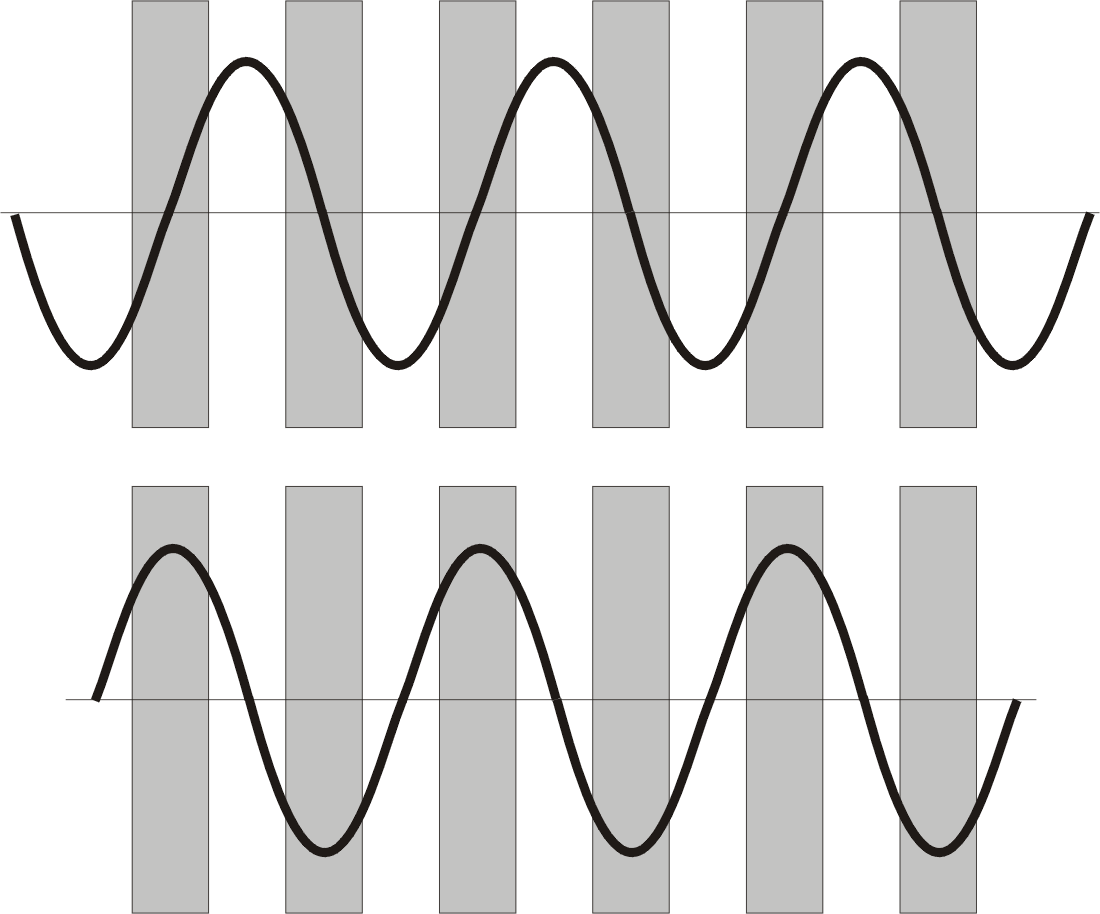
\includegraphics[width=7cm]{periodic/figures/field_placement}
\caption{Two ways to position the field: maximum intensity in the air (top) or in the dielectric (bottom). Note that this is a diagram in real space, i.e. the horizontal axis represents position.}
\label{fig-field-placement}
\end{figure}

Since in the low--frequency band the fields are more concentrated in the high dielectric, this band is usually called the \emph{dielectric band}. Often, the low dielectric is air, which explains why the upper band is often called the \emph{air band}.

All of this is completely analogous to semiconductor physics, where the periodicity of the semiconductor crystal gives rise to conduction and valence bands with a forbidden gap in between. In our case, we have artificial periodicity on a larger length scale (comparable to the wavelength of light used), so we call these structures \emph{photonic crystals}.

In the 1D case, the gap will start to close as soon as we move away from normal incidence. This is logical, as in the limiting case of grazing incidence, there is no longer periodicity in the propagation direction.

If we want to have a gap for oblique incidence too, we will need more--dimensional periodicity: carefully designed 2D structures can have a band gap for all propagation angles in a plane, whereas carefully designed 3D photonic crystals can have a gap for any propagation direction.

We say 'carefully designed structures' because in more dimensions it is not the case that any periodic structure will give rise to a band gap. This is in contrast with the 1D case, where a gap opens up for normal incidence as soon as there is any index contrast.

\section{2D and 3D periodic systems}

\subsection{Bloch's theorem in 3D}

The same principles we explained for 1D systems can of course be extended to higher dimensionalities.

By following a similar line of reasoning as in the 1D case, we can write down Bloch's theorem in three dimensions. For any eigenfunction ${\bf H}$ of $\Theta$ which describes a periodic system, there exists a vector ${\bf k}$ such that for any lattice vector ${\bf R}$ the following holds:

\begin{equation}
\fbox{$\displaystyle
{\bf H}_{\bf k} ({\bf r}+ {\bf R}) = e^{-j {\bf k} \cdot {\bf R}} {\bf H}_{\bf k} ({\bf r})
$}
\end{equation} 

Since we can label each solution by its wavevector, ${\bf k}$ was used a subscript of ${\bf H}$. 
Completely similar to the 1D argument, we can derive an alternative formulation of Bloch's theorem by saying that any solution ${\bf H}_{\bf k}$ can be written as

\begin{equation}
\fbox{$\displaystyle
{\bf H}_{\bf k} ({\bf r}) = e^{-j {\bf k} \cdot {\bf r}} {\bf u}_{\bf k} ({\bf r})
$}
\end{equation} 

The function ${\bf u}$ is periodic for all lattice vectors ${\bf R}$ of the crystal: ${\bf u}_{\bf k} ({\bf r} + {\bf R})  = {\bf u}_{\bf k} ({\bf r})$

\begin{sidebar}
\begin{ex}
By explicitly expanding in components, show that Bloch modes with wavevector $k$ satisfy the following equation:

$$\Theta_{\bf k} {\bf u}_{\bf k} = \omega^2 \mu {\bf u}_{\bf k}$$

with

$$\Theta_{\bf k} \stackrel{def}{=} (-j {\bf k} + \nabla) \times \left [ \frac{1}{\varepsilon({\bf r})}(-j{\bf k} +\nabla) \times \right ]$$

This formula can be used to build a numerical scheme to calculate Bloch modes: you first fix a value for ${\bf k}$ and then solve an eigenvalue problem, where the eigenvalues give the $\omega$--values where Bloch modes appear for this particular ${\bf k}$--value.

\end{ex}
\end{sidebar}

Just like in 1D, there is a range of ${\bf k}$--values which gives rise to non--redundant solutions which is called the Brillouin zone. However, in higher dimensions it is slightly more complicated to construct this region, so we will now spend some time discussing that.

\subsection{Reciprocal lattice}

Suppose we have a function $f({\bf r})$ that is periodic on a lattice, i.e. $f({\bf r} + {\bf R}) = f({\bf r})$ for all vectors ${\bf R}$ that translate the lattice into itself. As we have already seen, these vectors ${\bf R}$ are called the \emph{lattice vectors}.

Let us write down the continuous Fourier transform of the function $f$, which we can do for any sufficiently well--behaved function:

\begin{equation}
f({\bf r}) = \iiint g({\bf k}) e ^ {-j {\bf k} \cdot {\bf r}} d{\bf k}
\end{equation} 

Physically, this means we write $f$ as a sum of plane waves $e ^ {-j {\bf k} \cdot {\bf r}}$ with wavevectors ${\bf k}$ and expansion coefficients $g({\bf k})$.

An expansion like this can be performed on \emph{any} function. But $f$ is not just any function, it is periodic:

\begin{equation}
f({\bf r}) = \iiint g({\bf k}) e ^ {-j {\bf k} \cdot {\bf r}} d{\bf k} = f({\bf r} + {\bf R}) = \iiint g({\bf k}) e ^ {-j {\bf k} \cdot {\bf r}} e ^ {-j {\bf k} \cdot {\bf R}} d{\bf k}
\end{equation} 

From this, we can deduce that

\begin{equation}
g({\bf k}) = g({\bf k}) e ^ {-j {\bf k} \cdot {\bf R}}
\end{equation} 

But this is impossible, unless either $g({\bf k}) = 0$ or $e ^ {-j {\bf k} \cdot {\bf R}} = 1$. In other words, the transform $g$ is zero everywhere, except for discrete spikes at ${\bf k}$--values where $e ^ {-j {\bf k} \cdot {\bf R}} = 1$ for all ${\bf R}$.

So, what we have just discovered is that if we construct a periodic function using plane waves, we only need to consider those plane waves with wave vectors ${\bf k}$ such that $e ^ {-j {\bf k} \cdot {\bf R}} = 1$ for all lattice vectors ${\bf R}$. These ${\bf k}$--vectors are called the \emph{reciprocal lattice vectors} and are usually indicated by ${\bf G}$. They form a lattice of their own: i.e. adding two reciprocal lattice vectors yields another reciprocal lattice vector.

We still need to answer the question of how to build the set of all ${\bf G}$--vectors given the set of ${\bf R}$--vectors, i.e. find all ${\bf G}$ such that ${\bf G} \cdot {\bf R} = N 2 \pi$ for all ${\bf R}$ and for an integer $N$.

Every lattice vector ${\bf R}$ can be written as a linear combination of the so--called \emph{primitive lattice vectors}, which are the smallest vectors pointing from one lattice point to another. E.g. for a simple cubic lattice with spacing $a$, all ${\bf R}$s are of the form ${\bf R} = la {\bf 1}_x + ma {\bf 1}_y + na {\bf 1}_z$, with $(l,m,n)$ integers. In general, we call the primitive lattice vectors ${\bf a}_1$, ${\bf a}_2$ and ${\bf a}_3$. They don't need to be of unit length.

Since the reciprocal lattice vectors ${\bf G}$ also form a lattice, they have a set of primitive vectors ${\bf b}_i$ as well, such that ${\bf G} = l' {\bf b}_1 + m' {\bf b}_2 + n' {\bf b}_3$. Our requirement that ${\bf G} \cdot {\bf R} = N 2 \pi$ can now be written as

\begin{equation}
{\bf G} \cdot {\bf R} = ( l' {\bf b}_1 + m' {\bf b}_2 + n' {\bf b}_3) \cdot (l {\bf a}_1 + m {\bf a}_2 + n {\bf a}_3)  = N 2 \pi 
\end{equation} 

For all choices of $(l,m,n)$, this must hold for some $N$. We can satisfy this if we construct the ${\bf b}_i$ such that ${\bf a}_i \cdot {\bf b}_j = 2 \pi \delta_{ij}$, where $\delta_{ij}$ is non--zero only if $i=j$. We can do this by exploiting the fact that $ {\bf x} \cdot ({\bf x} \times {\bf y}) = 0$ for all vectors ${\bf x}$ and ${\bf y}$:

\begin{align}
{\bf b}_1 =& 2 \pi \frac{{\bf a}_2 \times {\bf a}_3}{{\bf a}_1 \cdot {\bf a}_2 \times {\bf a}_3} \nonumber \\
{\bf b}_2 =& 2 \pi \frac{{\bf a}_3 \times {\bf a}_1}{{\bf a}_1 \cdot {\bf a}_2 \times {\bf a}_3} \nonumber \\
{\bf b}_3 =& 2 \pi \frac{{\bf a}_1 \times {\bf a}_2}{{\bf a}_1 \cdot {\bf a}_2 \times {\bf a}_3}
\label{eq-recip}
\end{align} 

To summarise, when we build the Fourier transform of a periodic function, we only need to include plane waves with wave vectors that are reciprocal lattice vectors. To construct these reciprocal lattice vectors, we take the primitive lattice vectors and apply Eq.~\ref{eq-recip}.

\subsection{Brillouin zone in 3D}

We already know that for a Bloch mode there exists a vector ${\bf k}$ such that

\begin{equation}
{\bf H} ({\bf r}+ {\bf R}) = e^{-j {\bf k} \cdot {\bf R}} {\bf H} ({\bf r})
\end{equation} 

If ${\bf k}$ is incremented by a reciprocal lattice vector ${\bf G}$, then $e^{-j {\bf k} \cdot {\bf R}}$ is unchanged by the very definition of reciprocal lattice vector. So, incrementing ${\bf k}$ by ${\bf G}$ results in the same physical mode.

Therefore, we can restrict our attention to a region in ${\bf k}$--space where you cannot get from any point in that region to another in that region by adding a reciprocal lattice vector. This region is the Brillouin zone and consists of all the ${\bf k}$--vectors around the origin in reciprocal space that are closer to the origin than to any other neighbouring lattice point in the reciprocal lattice.

These two definitions are equivalent. If a particular ${\bf k}$ is closer to a neighbouring lattice point, you can always reach it by staying close to the original point and then translating it by the ${\bf G}$ that reaches from one lattice point to the other (Fig.~\ref{fig-bril-bisector}).

\begin{figure}
\centering
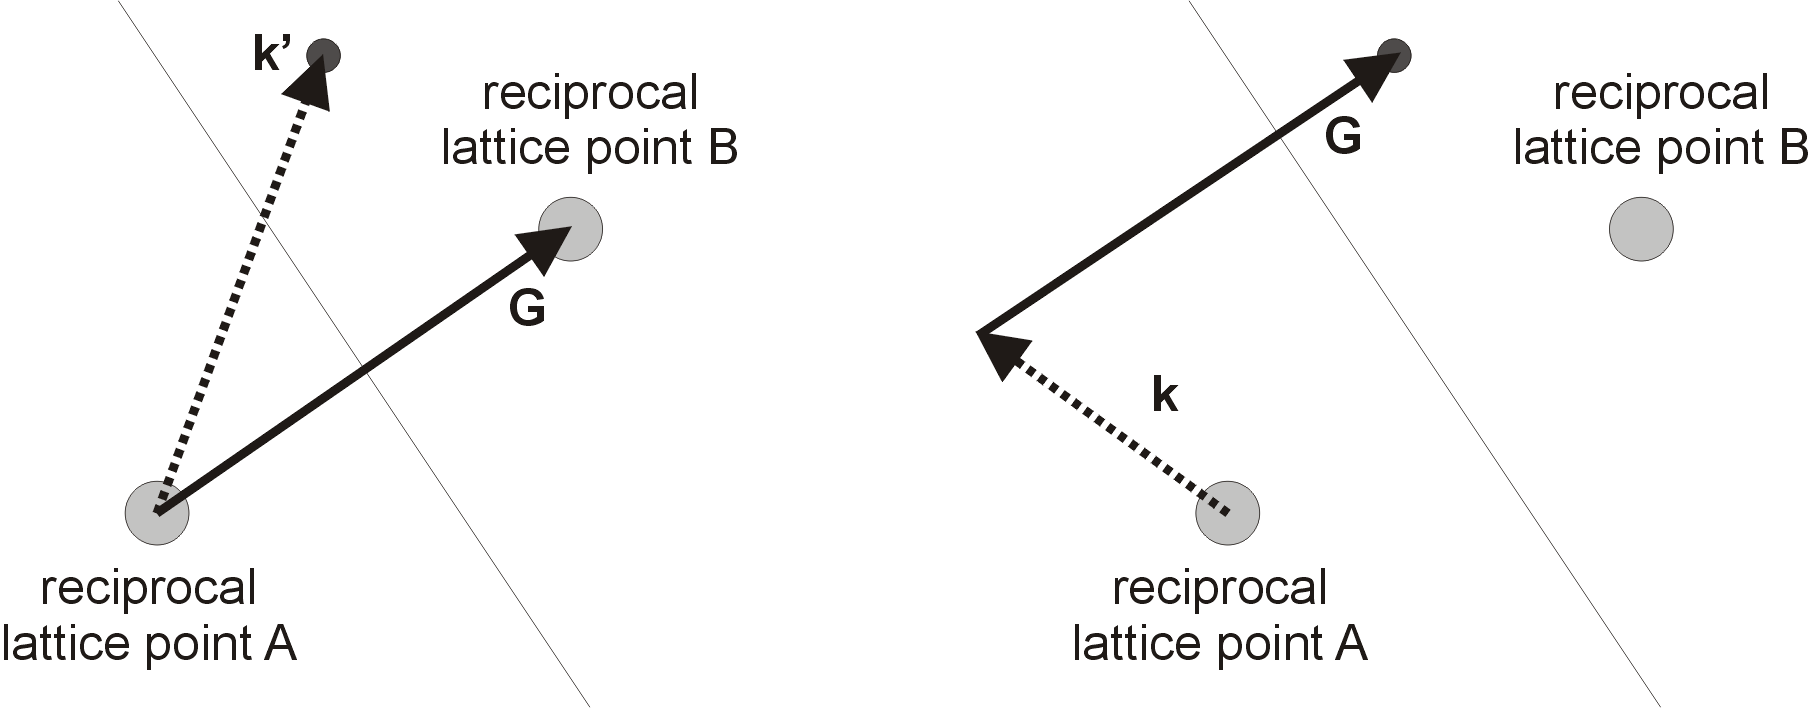
\includegraphics[width=11cm]{periodic/figures/bisector}
\caption{Construction of the Brillouin zone using bisectors of lines joining two lattice points. Any vector ${\bf k}'$ that reaches to an arbitrary point on the other side from $A$ can be expressed as the sum of a vector ${\bf k}$ on the same side and a lattice vector ${\bf G}$.}
\label{fig-bril-bisector}
\end{figure}

To make this more concrete, let's consider the case of a 2D square lattice (Fig.~\ref{fig-bril-square}). Its lattice vectors are ${\bf a}_1 = a {\bf 1}_x$ and ${\bf a}_2 = a {\bf 1}_y$. In order to use Eq.~\ref{eq-recip}, we need a third basis vector in the $z$--direction, but for that we can choose one of any length, since the structure is uniform in the $z$--direction. For the reciprocal lattice, we end up with  ${\bf b}_1 = 2 \pi / a {\bf 1}_x$ and ${\bf b}_2 = 2 \pi / a {\bf 1}_y$. So, the reciprocal lattice is also a square lattice, but with spacing $2 \pi / a$ instead of $a$.

To construct the Brillouin zone, we focus our attention on a particular point (the origin), and draw the lattice vectors that start at the origin. For each of these vectors, we draw the perpendicular bisectors, which divide the lattice into two half--planes (like in Fig.~ \ref{fig-bril-square}), one of which contains the origin. The intersection of all these half--planes forms the Brillouin zone (Fig.~\ref{fig-bril-square}).

\begin{figure}
\centering
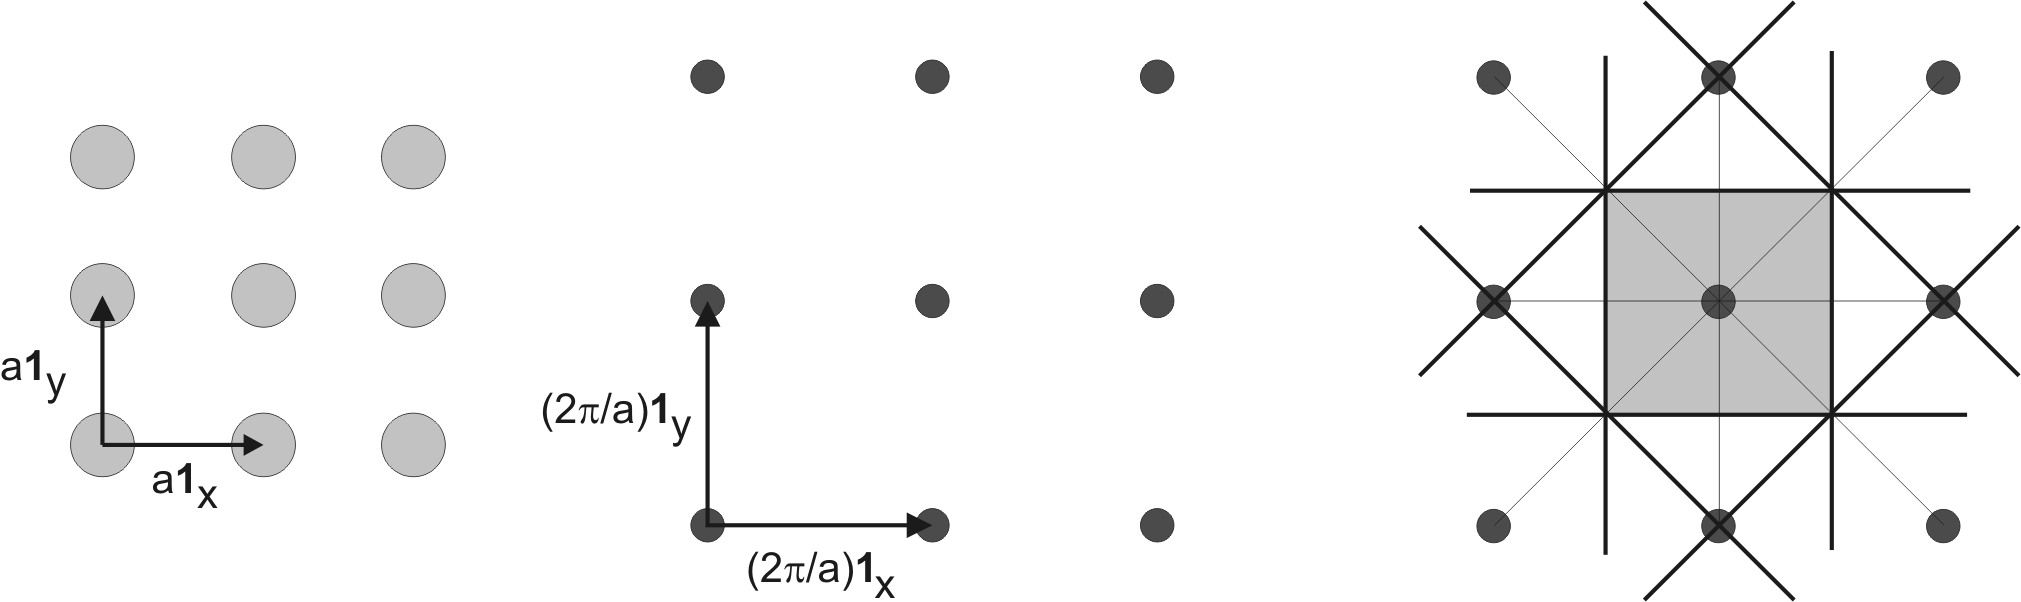
\includegraphics[width=12cm]{periodic/figures/brillouin_square}
\caption{The square lattice. Left: lattice in real space. Middle: lattice in reciprocal space. Right: construction of the Brillouin zone in reciprocal space.}
\label{fig-bril-square}
\end{figure}

\begin{sidebar}
\begin{ex}
For a triangular lattice, what are the lattice vectors, reciprocal lattice vectors and Brillouin zone?
\end{ex}
\end{sidebar}
 
\subsection{Irreducible Brillouin zone}

Often, a photonic crystal will have additional symmetries. E.g. the square lattice we considered earlier stays invariant for rotations over 90, 180 and 270 degrees. Another symmetry for the square crystal is mirror symmetry about the 45 degrees diagonal. The collection of symmetry operations (rotations, reflections, inversion) for which the crystal is invariant is called the \emph{point group} of the crystal.

All of these symmetries mean that there is additional redundancy in the Brillouin zone. The smallest region in the Brillouin zone for which the bands are not related by symmetry is called the \emph{irreducible Brillouin zone}. As shown in Fig.~\ref{fig-irred-bril}, the irreducible Brillouin zone for the square lattice is a triangular wedge $1/8$ the size of the full Brillouin zone. Also indicated in Fig.~\ref{fig-irred-bril} are some special high--symmetry points of the Brillouin zone. The origin is called the $\Gamma$--point, $X$ is in the direction along the shortest lattice vector and $M$ is in the direction of the diagonal. 

\begin{figure}
\centering
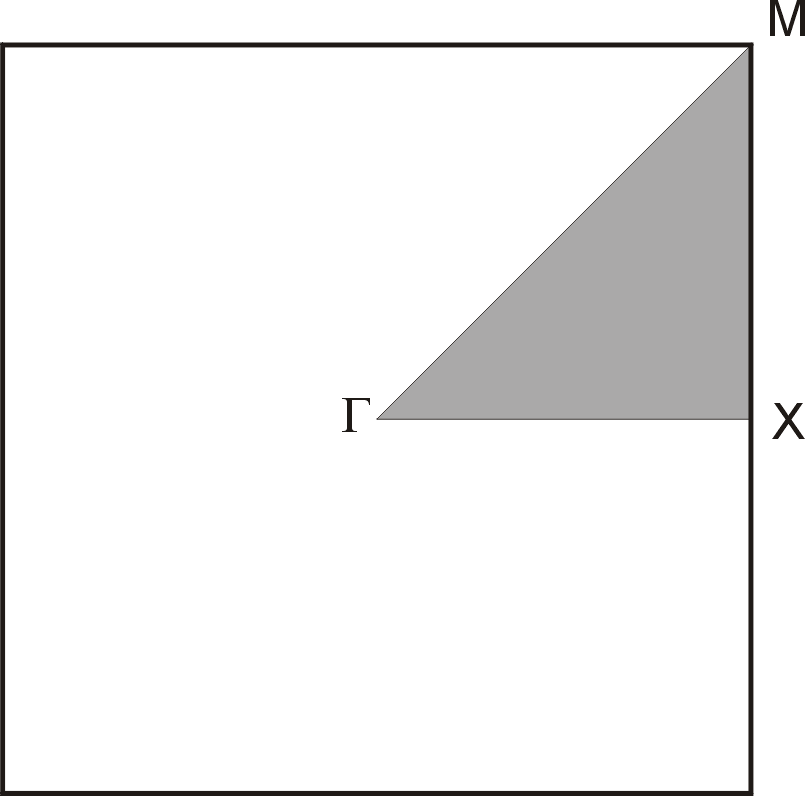
\includegraphics[width=4cm]{periodic/figures/irred_bril}
\caption{The irreducible Brillouin zone for the square lattice}
\label{fig-irred-bril}
\end{figure}

\subsection{Example: 2D square lattice of dielectric rods}

As an example we plot the band structure of a 2D square lattice of dielectric rods in air, for waves propagating in the $xy$--plane. For each ${\bf k}$--point in the triangular irreducible Brillouin zone there are a number of bands with increasing frequency. Each band can be plotted as a surface over the irreducible Brillouin zone, as illustrated in Fig.~\ref{fig-bands-rods-3D}:

\begin{figure}
\centering
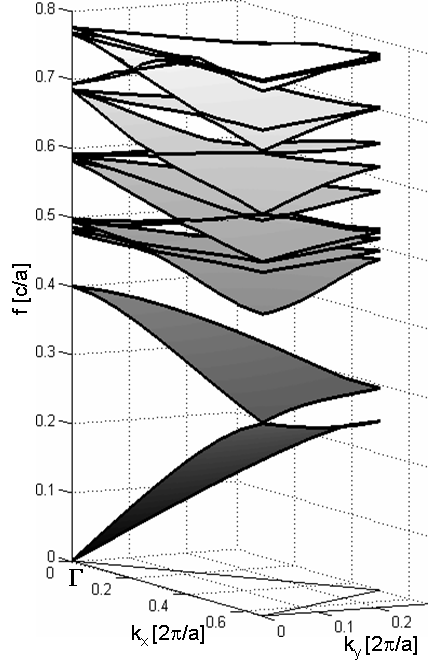
\includegraphics[width=5cm]{periodic/figures/3d_bands}
\caption{Full TM band diagram for a square lattice of dielectric rods, as a set of surfaces in $k$--space.}
\label{fig-bands-rods-3D}
\end{figure}

As such a 3D plot quickly becomes difficult to interpret, people usually only plot the bands along the edges of the irreducible Brillouin zone, as is done in Fig.~\ref{fig-bands-rods}. We can see that there is a bandgap for modes with TM polarisation, but not for TE. In the context of photonic crystals, TM is defined as modes with the ${\bf E}$--vector along the rods in the $z$--direction.

\begin{figure}
\centering
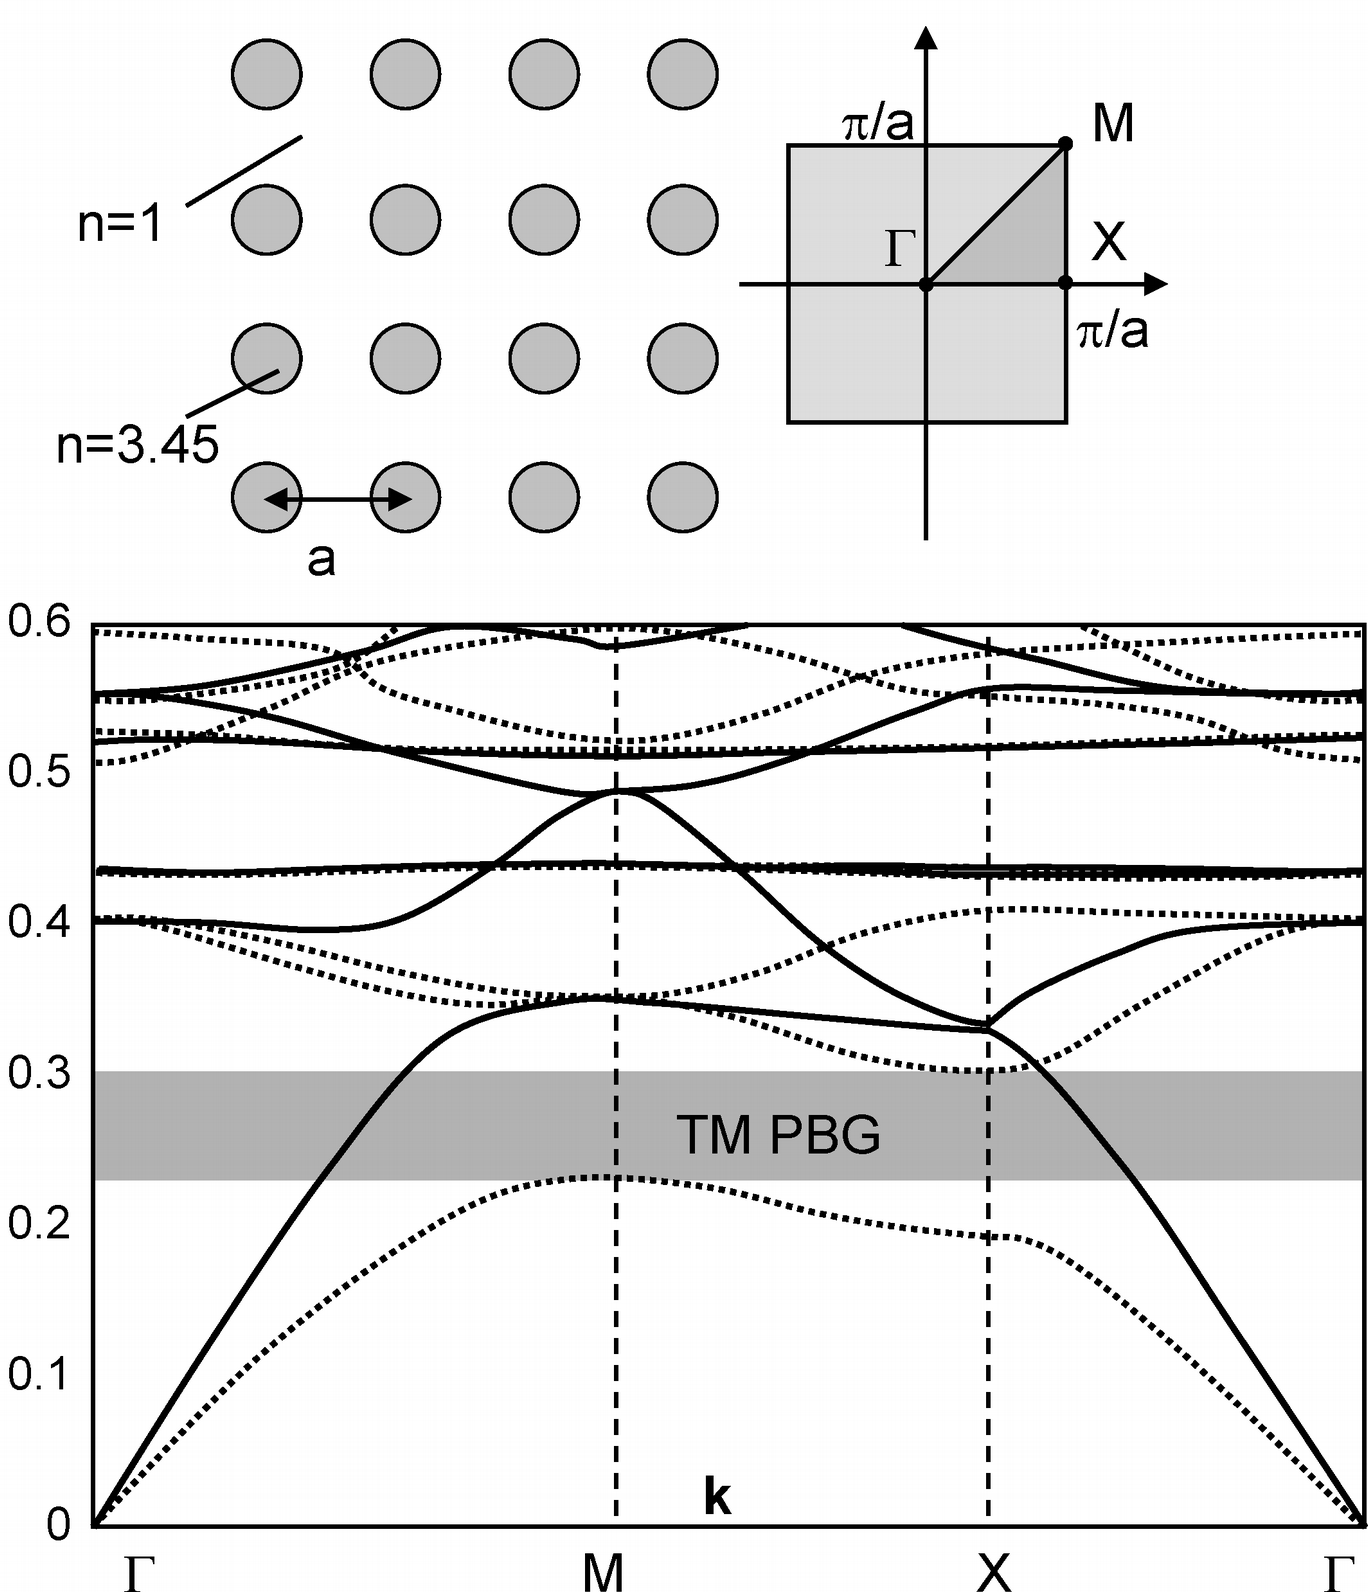
\includegraphics[width=7cm]{periodic/figures/square_bands}
\caption{Projected band diagram for a square lattice of dielectric rods. Dotted band are TM, full lines are TE polarisation.}
\label{fig-bands-rods}
\end{figure}

\begin{sidebar}
\begin{ex}
For a 2D square lattice of dielectric rods, some solutions will be polarised with the electric field parallel to the rods, and some modes will have the electric field perpendicular to the rods. For both situations, calculate the ratio of the electric energy $\epsilon |E|^2$ just inside and just outside the rods. In which case will the electric field be more confined in the rods?
\end{ex}
\end{sidebar}
 

\subsection{Time reversal symmetry}

\begin{sidebar}
\begin{ex}
Band diagrams are symmetric around $k=0$, i.e. if there is a mode at frequency $\omega$ with wave vector $k$, there is always a mode at that same frequency with wave vector $-k$. This is true even if the crystal itself does not have inversion symmetry. The mode at $-k$ can be thought of as the backward version of the mode at $k$ and is a consequence of the time reversal symmetry of Maxwell's equations. Make this plausible by taking the following steps:
\begin{itemize}
\item Using the definition of phasors, show that if $H_x$ is the phasor corresponding to $ H_{x,0} \cos \left( \omega t + \phi \right)$, then the phasor $H^*_x$ corresponds to the time-reversed signal $ H_{x,0} \cos \left(- \omega t + \phi  \right)$.
\item Show that for lossless systems ${\bf H}^*$ is also a eigenfunction if ${\bf H}$ is an eigenfunction. What is its eigenvalue?
\item From the second form of Bloch's theorem, associate ${\bf H}^*$ with a Bloch mode at $-k$. What is its corresponding ${\bf u}$ function?
\end{itemize}

\end{ex}
\end{sidebar}

\section{Applications of photonic crystals}

Just as with semiconductors, photonic crystals only become truly useful when defects are introduced in the crystal lattice (Fig.~\ref{fig-defects}).

\begin{figure}
\centering
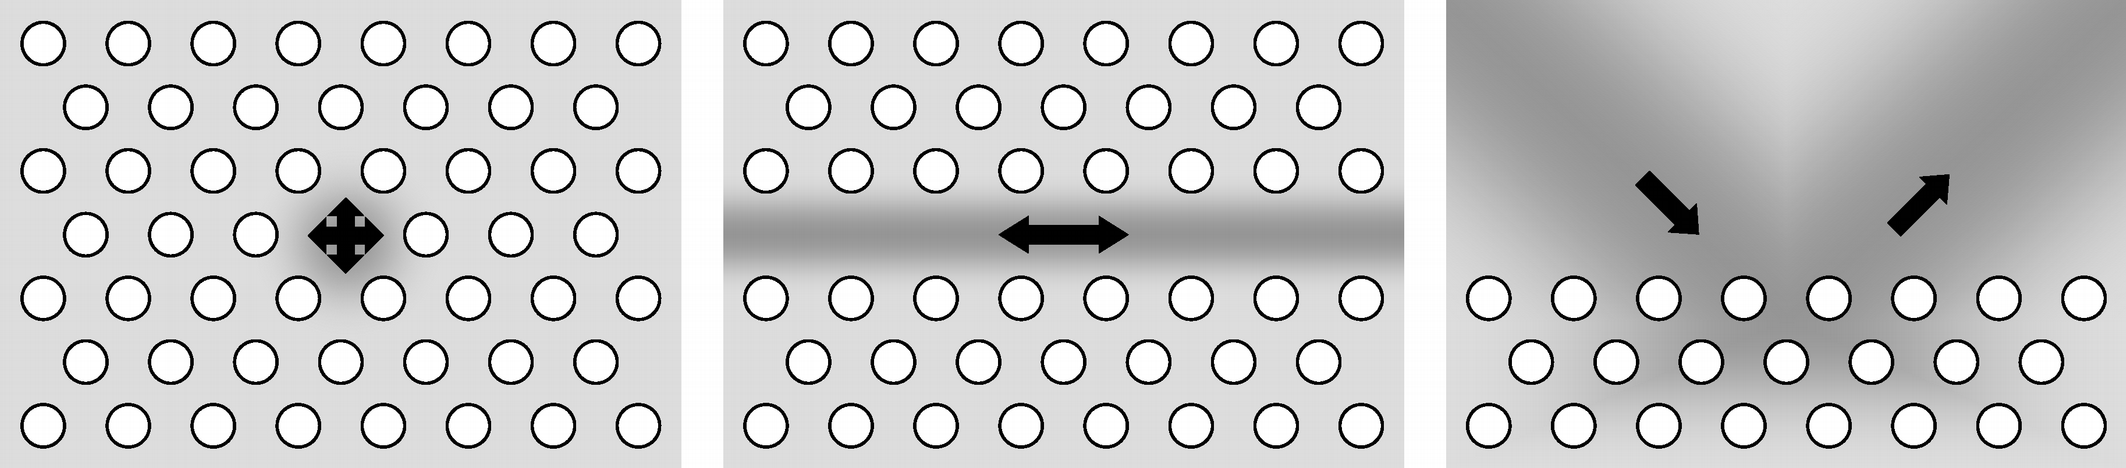
\includegraphics[width=10cm]{periodic/figures/2d_defects}
\caption{Defects in a photonic crystal: a) point defect b) line defect c) surface defect }
\label{fig-defects}
\end{figure}

When we introduce a point defect in a crystal, we create a small region of space which is surrounded by a photonic crystal which acts as a perfect reflector. So, light has no way to escape from this region and we have created a resonating \emph{cavity}.

Similarly, when we create a line defect, light cannot propagate into the crystal and therefore it has no choice but to follow the line defect. In this way, we have created a \emph{waveguide}.

Finally, we can also create a surface defect, where we just exploit the \emph{mirror} properties  of the photonic crystal.

The nice thing about these structures is that they are very small, on the order of the wavelength of the light used. This is why they are often called \emph{nanophotonic} structures. They offer the possibility of miniaturising and integrating a variety of optical components (like e.g. the bends, splitters and filters from Fig.~\ref{fig-components}) onto a single photonic IC.

\begin{figure}
\centering
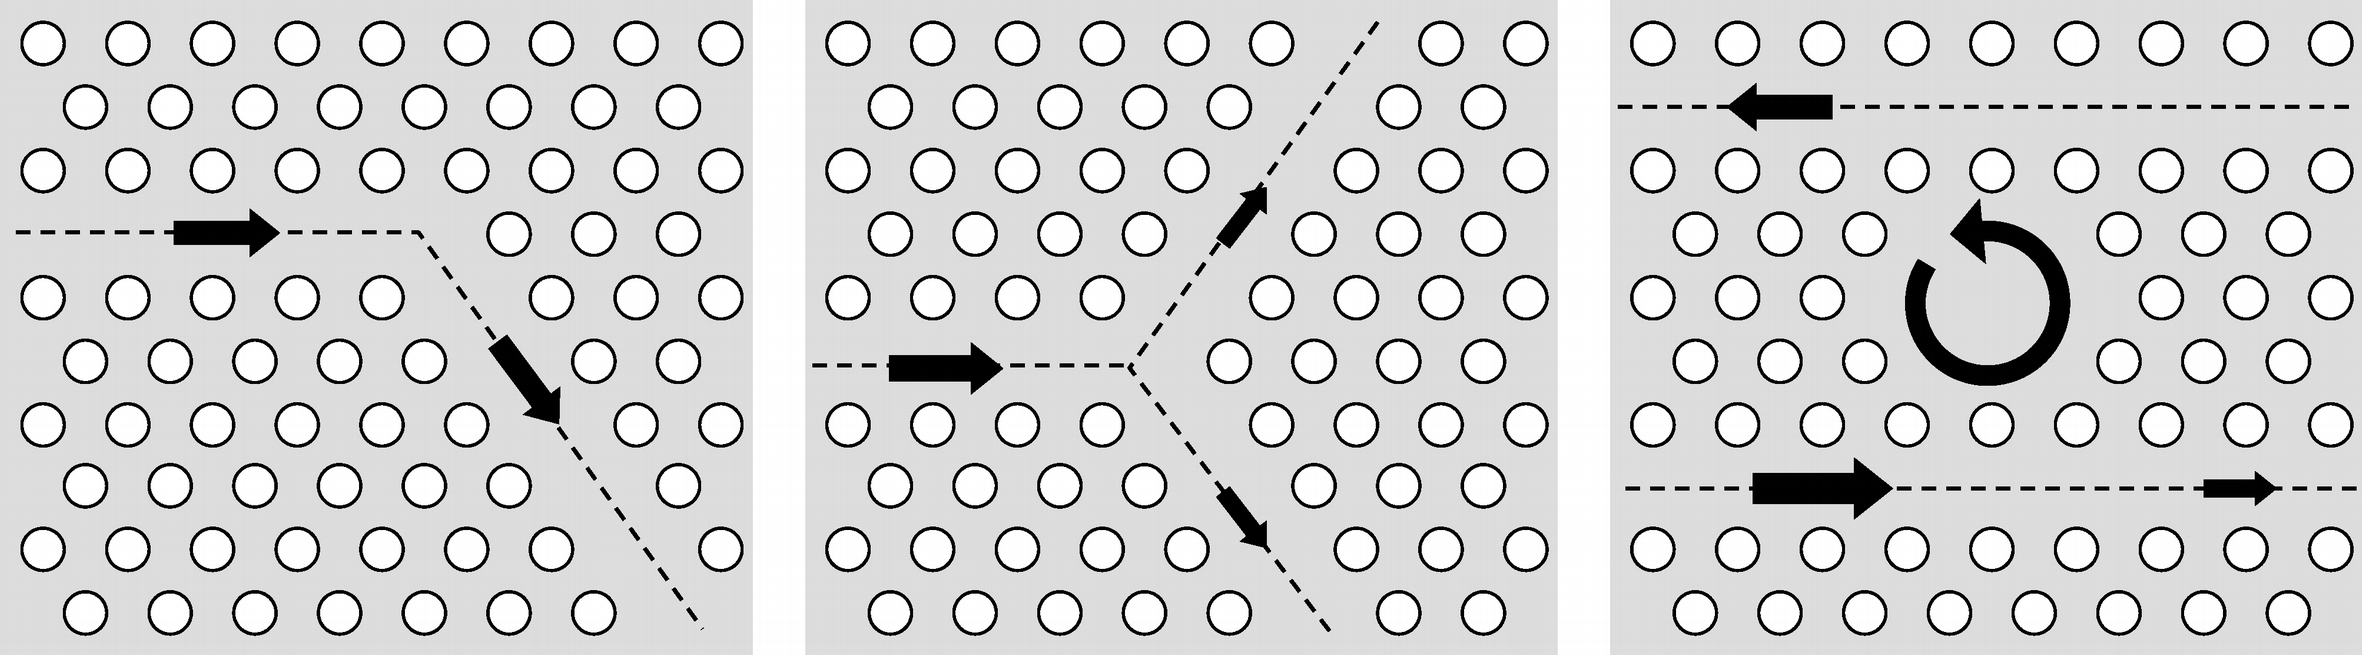
\includegraphics[width=10cm]{periodic/figures/2d_components}
\caption{Example of photonic crystal components: a) bend b) splitter c) resonant filter}
\label{fig-components}
\end{figure}

\pagebreak
\section*{Felix Bloch (1905--1983)}

\parpic{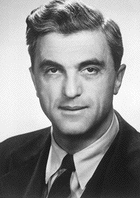
\includegraphics{periodic/figures/bloch}}

Felix Bloch was born in Zurich, Switzerland, on October 23, 1905, as the son of Gustav Bloch and Agnes Bloch. From 1912 to 1918 he attended the public primary school and subsequently the "Gymnasium" of the Canton of Zurich, which he left in the fall of 1924 after having passed the "Matura", i.e. the final examination which entitled him to attend an institution of higher learning.
 
Planning originally to become an engineer, he entered directly the Federal Institute of Technology (ETH) in Zurich. After one year's study of engineering he decided instead to study physics, and changed therefore over to the Division of Mathematics and Physics at the same institution. During the following two years he attended, among others, courses given by Debye, Scherrer, Weyl, as well as Schr\"{o}dinger, who taught at the same time at the University of Zurich and through whom he became acquainted, toward the end of this period, with the new wave mechanics. Bloch's interests had by that time turned toward theoretical physics. After Schr\"{o}dinger left Zurich in the fall of 1927 he continued his studies with Heisenberg at the University of Leipzig, where he received his degree of Doctor of Philosophy in the summer of 1928 with a dissertation dealing with the quantum mechanics of electrons in crystals and developing the theory of metallic conduction. Various assistantships and fellowships, held in the following years, gave him the opportunity to work with Pauli, Kramers, Heisenberg, Bohr, and Fermi, and to further theoretical studies of the solid state as well as of the stopping power of charged particles.
 
Upon Hitler's ascent to power, Bloch left Germany in the spring of 1933, and a year later he accepted a position which was offered to him at Stanford University. The new environment in which he found himself in the United States helped toward the maturing of the wish he had had for some time to undertake also experimental research. Working with a very simple neutron source, it occurred to him that a direct proof for the magnetic moment of the free neutrons could be obtained through the observation of scattering in iron. In 1936, he published a paper in which the details of the phenomenon were worked out and in which it was pointed out that it would lead to the production and observation of polarised neutron beams. The further development of these ideas led him in 1939 to an experiment, carried out in collaboration with L.W. Alvarez at the Berkeley cyclotron, in which the magnetic moment of the neutron was determined with an accuracy of about one percent.
 
During the war years Dr. Bloch was also engaged in the early stages of the work on atomic energy at Stanford University and Los Alamos and later in counter--measures against radar at Harvard University. Through this latter work he became acquainted with the modern developments of electronics which, toward the end of the war, suggested to him, in conjunction with his earlier work on the magnetic moment of the neutron, a new approach toward the investigation of nuclear moments.
 
These investigations were begun immediately after his return to Stanford in the fall of 1945 and resulted shortly afterward in collaboration with W.W. Hansen and M.E. Packard in the new method of nuclear induction, a purely electromagnetic procedure for the study of nuclear moments in solids, liquids, or gases. A few weeks after the first successful experiments he received the news of the same discovery having been made independently and simultaneously by E.M. Purcell and his collaborators at Harvard.
 
Most of Bloch's work in the subsequent years has been devoted to investigations with the use of this new method. In particular, he was able, by combining it with the essential elements of his earlier work on the magnetic moment of the neutron, to remeasure this important quantity with great accuracy in collaboration with D. Nicodemus and H.H. Staub (1948). His more recent theoretical work has dealt primarily with problems which have arisen in conjunction with experiments carried out in his laboratory.

In 1952 he was awarded the Nobel prize in Physics, together with Purcell, "for their development of new methods for nuclear magnetic precision measurements and discoveries in connection therewith".
 
In 1954, Bloch took a leave of absence to serve for one year as the first Director General of CERN in Geneva. After his return to Stanford University he continued his investigations on nuclear magnetism, particularly in regard to the theory of relaxation. In view of new developments, a major part of his recent work deals with the theory of superconductivity and of other phenomena at low temperatures.
 
In 1961, he received an endowed Chair by his appointment as Max Stein Professor of Physics at Stanford University.
 
Prof. Bloch married in 1940 Dr. Lore Misch, a refugee from Germany and herself a physicist.

(From Nobel Lectures. Physics 1942--1962, Elsevier Publishing Company, Amsterdam, 1964)

